\section{Results}
\label{sec:results}

%In this section, we discuss our experimental results on both simulated and biological datasets. We conduct extensive experiments with 10 replicates of 100-taxon simulated dataset, two biological rRNA datasets and 27 BAliBASE datasets. We begin by picking two sets of objective functions by analyzing the generated set of alignments based on resultant tree quality. Then for all datasets, we compare the alignments generated by those objective sets with nine state-of-the-art tools. 

We conducted extensive experiments with both simulated and biological datasets. We begin by carefully and systematically selecting two multi-objective formulations which are potentially useful for phylogenetic tree estimation employing NSGA-III and multiple linear regression. Next, we generate alignments through running NSGA-II as well as nine state-of-the-art MSA tools. Then we compare those alignments with respect to both generic and domain specific quality measures. In this section, we discuss our obtained results after introducing our chosen datasets. In what follows, unless otherwise specified, when we discuss the (best) results of a tool, we mean one of the above-mentioned nine tools.

\begin{comment}
\begin{figure*}[!htbp]
\centering
\begin{adjustwidth}{-0.5cm}{-0.5cm}
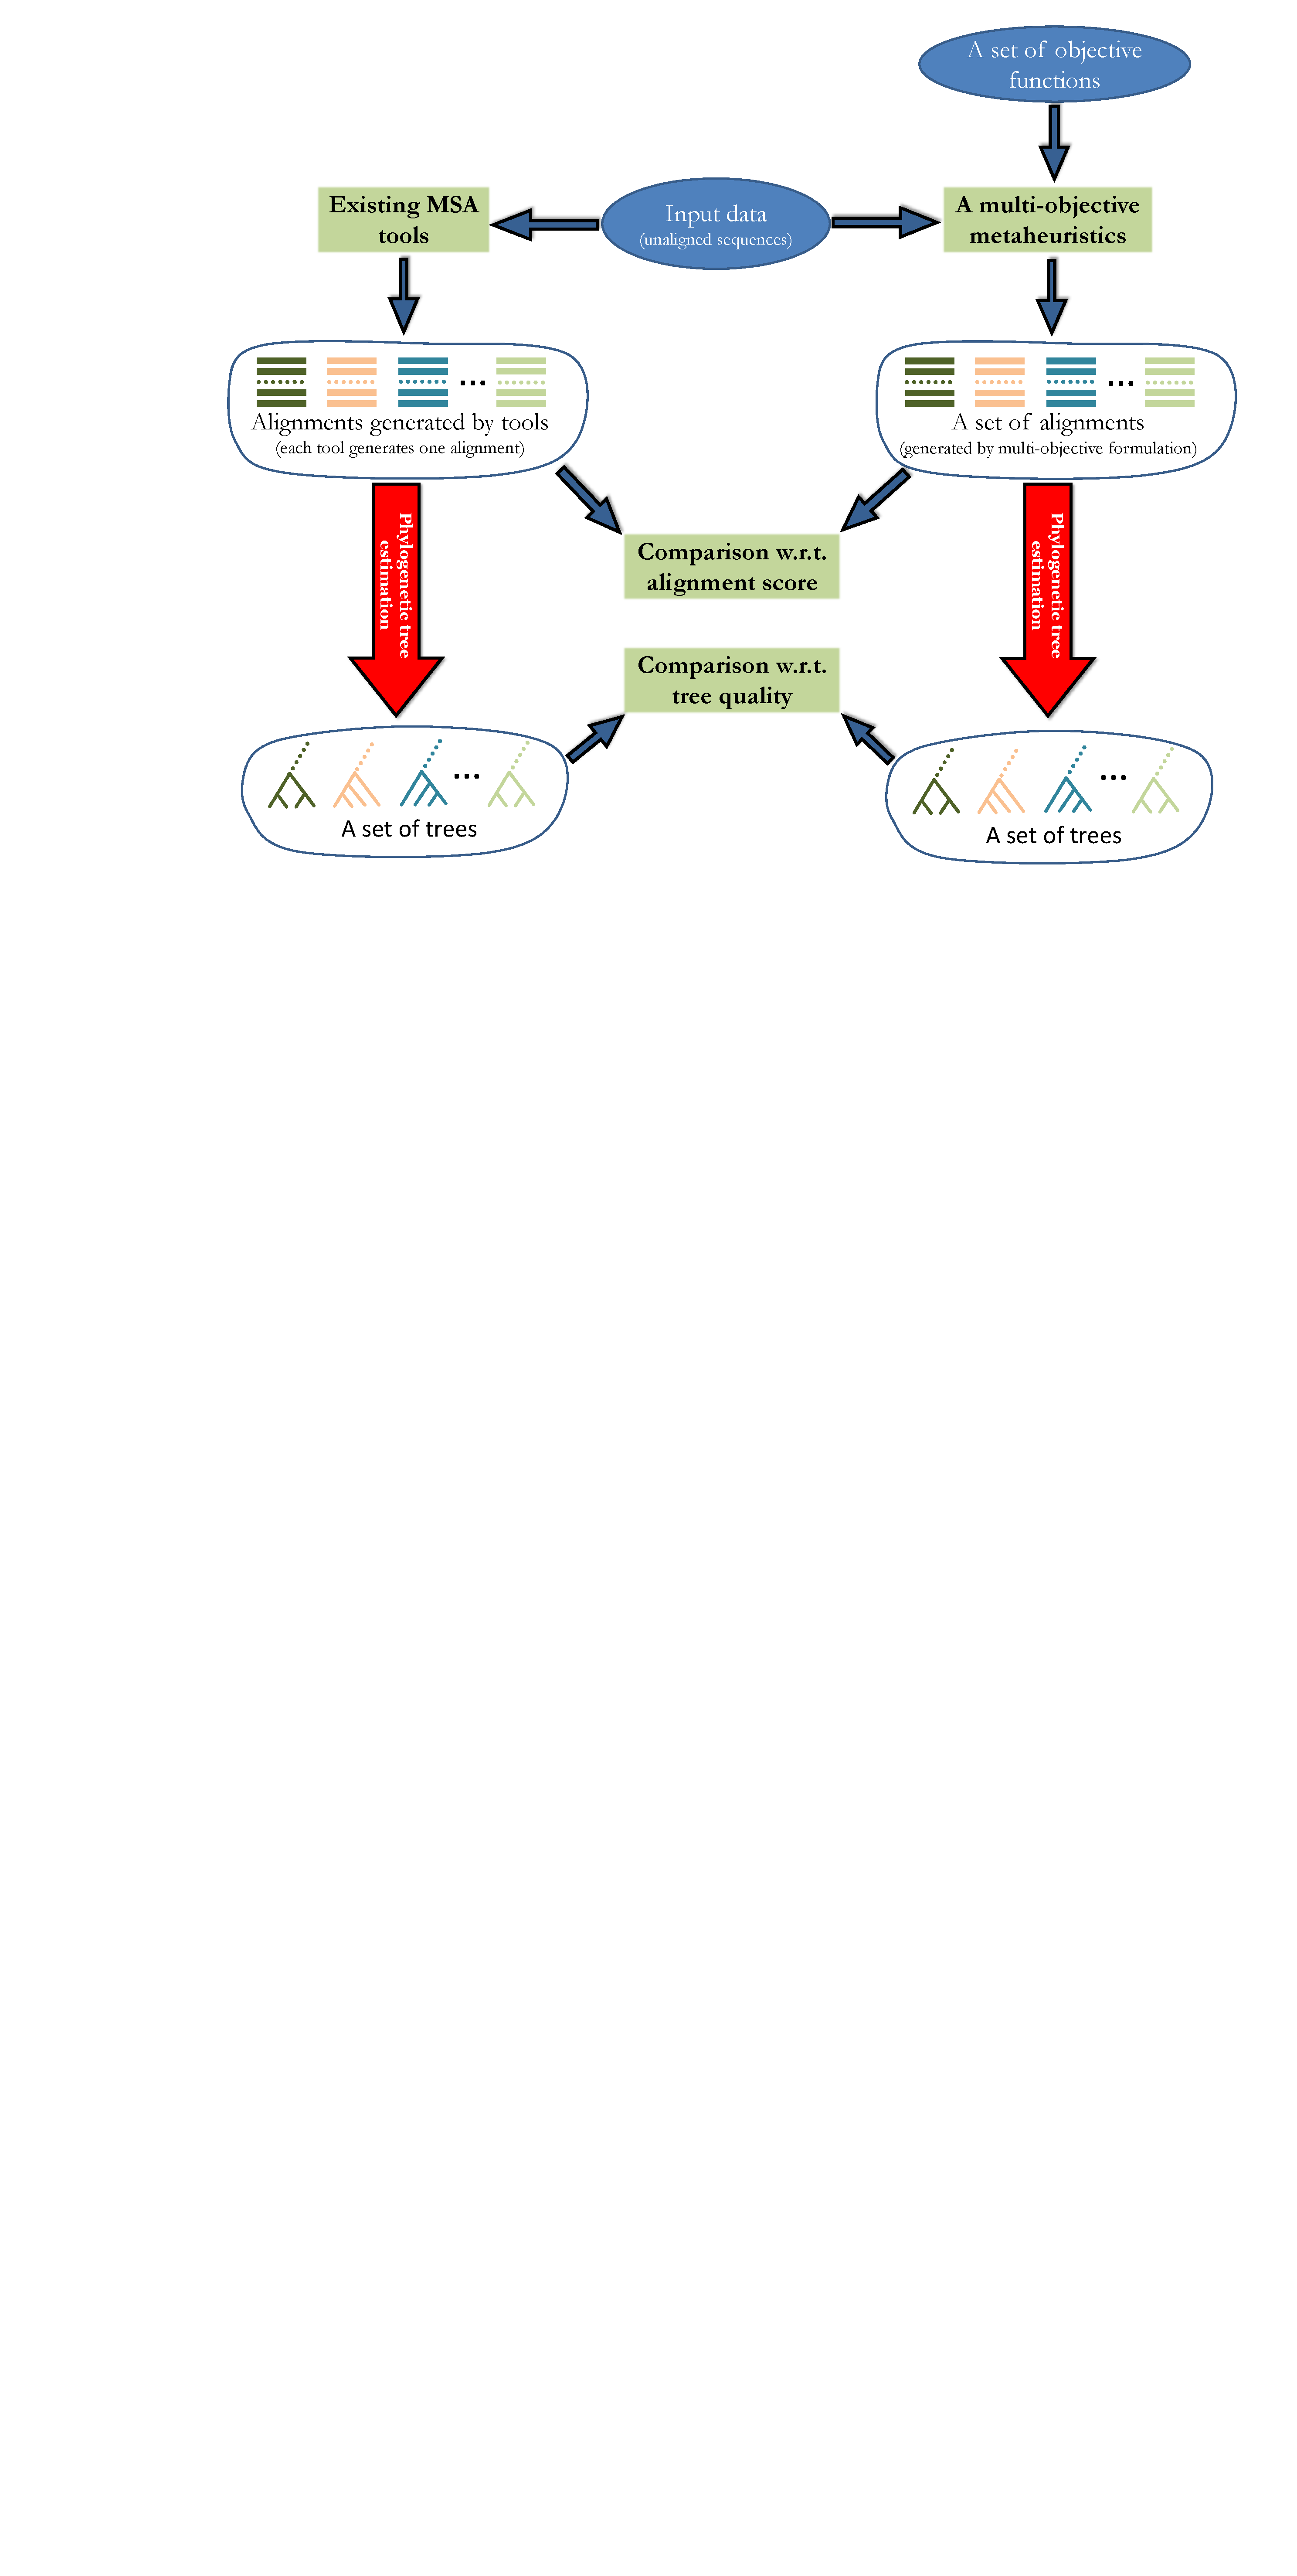
\includegraphics[width=1.1\textwidth]{Figure/pipeline}
\caption{Our methodology for finding the impact of a multi-objective formulation (i.e., a set of objective functions) of MSA on phylogenetic tree estimation. For each dataset (i.e., unaligned sequences), we run a multi-objective metaheuristic. It simultaneously optimizes the given objective functions and outputs a set of alignments which represents the best-possible compromise among all objective functions. We also run several existing MSA tools on that dataset and each tool generates one alignment. We evaluate the quality of each generated alignments with respect to the reference alignments using widely used scores. Also we estimate phylogenetic trees for all alignments and evaluate each tree with respect to the reference. Then we compare the alignments and the corresponding phylogenetic trees generated by the multi-objective formulation with the ones generated by the existing tools based on alignment score as well as tree quality. We also observe the association between alignment scores and tree quality values to examine whether it is appropriate to use alignment score in the context of phylogeny estimation.}
\label{fig:pipeline}
\end{adjustwidth}
\end{figure*}

\subsection{Experimental design}
Our experimental methodology is briefly described below (please see also Figure~\ref{fig:pipeline}):
\begin{itemize}
\item \underline{Step 1:} Following a systematic approach involving multiple linear regression applied on a simulated dataset, we first make an attempt to identify and choose two multi-objective formulations that turn out to be potentially more effective in the context of phylogeny estimation. 
\item \underline{Step 2:} We run a popular and effective multi-objective metaheuristics on both biological and simulated datasets to optimize each set of objective functions selected in Step 1. Each run of the metaheuristics on each dataset gives us a set of alignments as output. 
\item \underline{Step 3:} We also run nine state-of-the-art MSA tools (please see Section~\ref{sec:methods}, Table~\ref{tab:msa_tools}) to generate alignments on all these datasets.
% \comment{with default parameters. It is the usual practice of MSA literature. Should I exclude this?} and then estimate maximum likelihood (ML) phylogenetic tree from those alignments. We evaluate the quality of these alignments and ML trees.
\item \underline{Step 4:} We evaluate the quality of each generated alignment with respect to the reference alignment using two popular measures, namely, SP score and TC score. 
%For biological datasets, we used manually curated alignments as reference.
\item \underline{Step 5:} For each of the generated alignments, we infer maximum likelihood (ML) phylogenetic tree. Then we measure the quality of each inferred tree with respect to the reference tree (true tree) using the mostly used measure in the literature called false negative (FN) rate.
\item \underline{Step 6:} Finally we compare the alignments and the corresponding ML trees generated by the multi-objective optimization with the ones generated by the state-of-the-art tools. % using statistical measures.
\end{itemize}
\end{comment}

\subsection{Datasets}
%We aim to validate the effectiveness of an objective function in terms of how it can help to estimate the phylogenetic tree. So, in this context, a good objective function has good statistical evidence of leading to good trees. To conduct our study we require knowledge of the true phylogenetic tree which can be used as a reference for measuring the goodness of estimated trees. 
We studied a simulated dataset (100-taxon simulated dataset~\citep{liu2009rapid}) as well as two biological datasets (biological rRNA datasets~\citep{liu2009rapid} and BAliBASE 3.0 benchmark~\citep{thompson2005balibase}). As the simulated dataset comes with the true phylogenetic tree, we use this dataset to examine whether a multi-objective formulation of MSA is potentially application-aware and in the sequel, we select two such formulations somewhat similar to the training phase of a machine learning approach. Afterwards, we validate the effectiveness of the selected formulations against the state-of-the-art MSA tools based on biological datasets.  
% We now briefly introduce them in this subsection.   

From the 100-taxon simulated dataset, we randomly selected five replicates. And among the biological datasets, we chose two challenging ribosomal RNA datasets along with 27 random instances of the widely used BAliBASE 3.0 benchmark. Section~\ref{sec:dataset_stat} of the supplementary file provides a detailed description of these datasets. 

\begin{comment}
\subsubsection{100-taxon simulated dataset}
We used 10 (out of 20) randomly selected replicates (R0, R2, R4, R6, R9, R10, R13, R14, R17, R19) of simulated nucleotide dataset from the study of~\citealp{liu2009rapid}. It is publicly available at \url{https://sites.google.com/eng.ucsd.edu/datasets/sate-i}. Table~\ref{tab:sim_stat} in the supplementary file gives the reference alignment statistics for this dataset.
% generated from a model tree (can be used as true tree) with model condition (100 taxa, short gap length type)



% Table generated by Excel2LaTeX from sheet 'Sheet1'
\begin{table}[htbp]
\centering
\caption{Reference alignments for 100-taxon simulated dataset.}
\begin{tabular}{|l|r|}
\hline
\multicolumn{1}{|c|}{Feature} & \multicolumn{1}{c|}{Value} \\
\hline
Number of taxa & 100 \\
\hline
Number of sites & 1698.2 \\
\hline
Percent indels & 40.4 \\
\hline
Avg. gap length & 3.1 \\
\hline
\end{tabular}%
\label{tab:sim_stat}%
\end{table}%


\subsubsection{Biological rRNA datasets}
We analyzed two biological ribosomal RNA datasets, 23S.E and 23S.E.aa\_ag, from~\citealp{liu2009rapid} which are challenging for phylogeny estimation methods. Each of these datasets is given with a highly reliable, curated reference alignment from Gutell Lab. The statistics of the reference alignments of these datasets are presented in Table~\ref{tab:bio_stat} of the supplementary file. Reference trees for these datasets were generated from the reference alignments by running RAxML~\citep{stamatakis2014raxml} with bootstrapping, and retaining only the highly supported edges. We evaluated generated alignments with respect to the reference alignment using the tool FastSP \citep{mirarab2011fastsp}.

\begin{comment}

% Table generated by Excel2LaTeX from sheet 'Sheet2'
\begin{table}[htbp]
\small
\centering
\caption{Reference alignments for two biological rRNA datasets.}
\begin{tabular}{|l|r|r|}
\hline
\multicolumn{1}{|c|}{Feature} & \multicolumn{1}{c|}{23S.E.aa\_ag} & \multicolumn{1}{c|}{23S.E} \\
\hline
Number of taxa & 144   & 117 \\
\hline
Number of sites & 8,619 & 9,079 \\
\hline
Percent indels & 61.1  & 59.7 \\
\hline
Avg. gap length & 13.5  & 12.6 \\
\hline
\end{tabular}%
\label{tab:bio_stat}%
\end{table}%



\subsubsection{BAliBASE datasets}
BAliBASE 3.0 \citep{thompson2005balibase} is the most widely used benchmark alignment databases of protein families. It provides manually refined reference alignments of high quality based on 3D structural superposition. These datasets are organized into six groups according to their families and similarities: \commentA{RV11 (very divergent sequences, residue identity below 20\% ), RV12 (medium to divergent sequences, 20\%-40\% residue identity), RV20 (families with one or more highly divergent sequences), RV30 (divergent subfamilies), RV40 (sequences with large terminal N/C extensions), and RV50 (sequences with large internal insertions).} In this study, we selected four to five representative datasets from each group as reported in Table~\ref{tab:balibase} of the supplementary file. We generated reference trees for these datasets by running RAxML with bootstrapping. We evaluated estimated alignments with respect to the core blocks (regions for which reliable alignments are known to exist) using the program bali\_score available at~\url{http://www.lbgi.fr/balibase/BalibaseDownload/}.
% We randomly take 27 (out of 218) datasets (Table~\ref{tab:balibasel})

\begin{comment}

% Table generated by Excel2LaTeX from sheet 'Sheet2'
\begin{table}[htbp]
\small
\centering
\caption{ BAliBASE datasets selected for this study.}
\begin{tabular}{|l|L{5.1cm}|}
\hline
\multicolumn{1}{|c|}{Group} & \multicolumn{1}{c|}{Datasets selected} \\
\hline
RV11  & BB11005, BB11018, BB11020, BB11033 \\
\hline
RV12  & BB12001, BB12013, BB12022, BB12035, BB12044 \\
\hline
RV20  & BB20001, BB20010, BB20022, BB20033, BB20041 \\
\hline
RV30  & BB30002, BB30008, BB30015, BB30022 \\
\hline
RV40  & BB40001, BB40013, BB40025, BB40038, BB40048 \\ %
\hline
RV50  & BB50001, BB50005, BB50010, BB50016 \\
\hline
\end{tabular}%
\label{tab:balibase}%
\end{table}%
\end{comment}

\subsection{Selection of appropriate multi-objective formulations}
\label{sec:selection_msa_formulation}
%We choose two sets of objective functions (i.e. multi-objective formulation) to conduct experiments based on this dataset. We select the first set of objective functions from among three existing studies based on their relative performance in the context of phylogeny estimation. Afterwards, we follow a similar approach to form the second set by incorporating our proposed objective functions. Now we discuss the selection process of these two sets along with their performance on this dataset.
As has been mentioned above, we have used 100-taxon simulated dataset to select one or more multi-objective formulations that have the potential to be ``application-aware''. We first conduct extensive experiments to choose a formulation (i.e., a set of objective functions) of MSA from among the existing popular ones from the literature (Section~\ref{sec:existing_msa_formulation}); subsequently, we also suggest a new promising formulation (Section~\ref{sec:new_msa_formulation}).  
%We use this dataset to select a potentially application-aware multi-objective formulation (i.e., a set of objective functions) of MSA from the literature. Then based on the same dataset we present a new promising formulation. We perform these steps by adopting a novel methodology based on the careful application of multiple linear regression. Now we discuss the selection process of these two formulations followed by their performance against the state-of-the-art tools.
%At the end, we compare these two objective set based on their performance on 10 replicates.
\begin{comment}

\begin{figure*}[!htbp]    
\begin{adjustwidth}{-1cm}{-1cm}
\centering
\begin{subfigure}{0.35\textwidth}
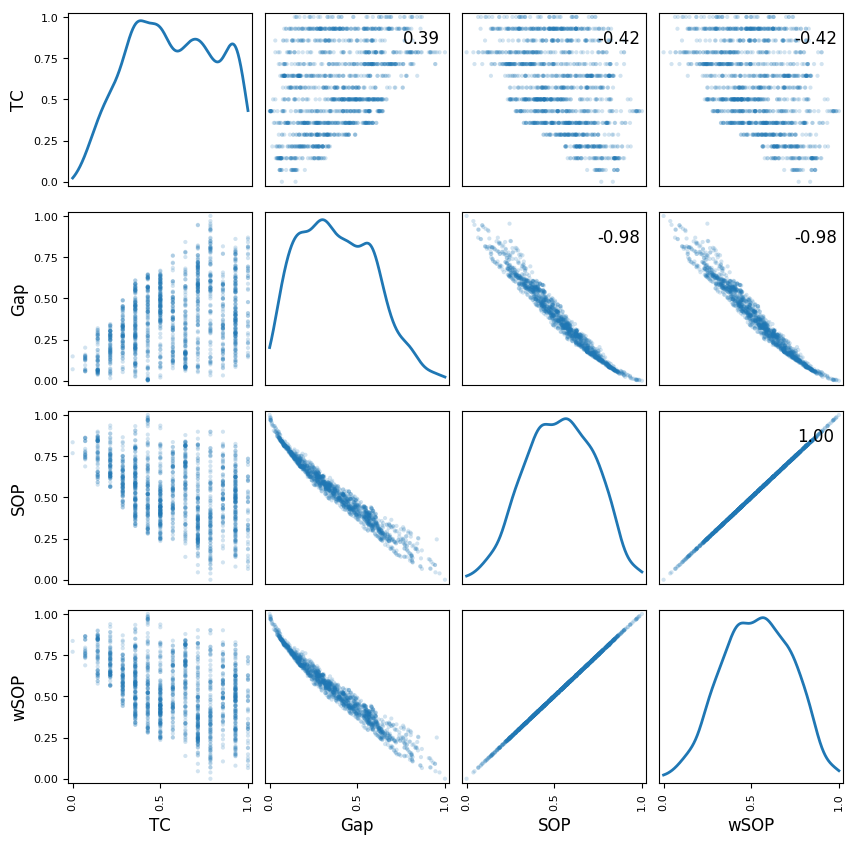
\includegraphics[width=\columnwidth]{Figure/NumGaps_SOP_TC_wSOP/precomputedInit/R0/fig/scatter_mattrix}
\caption{R0}
%\label{fig:con_pr09}
\end{subfigure}    
\begin{subfigure}{0.35\textwidth}
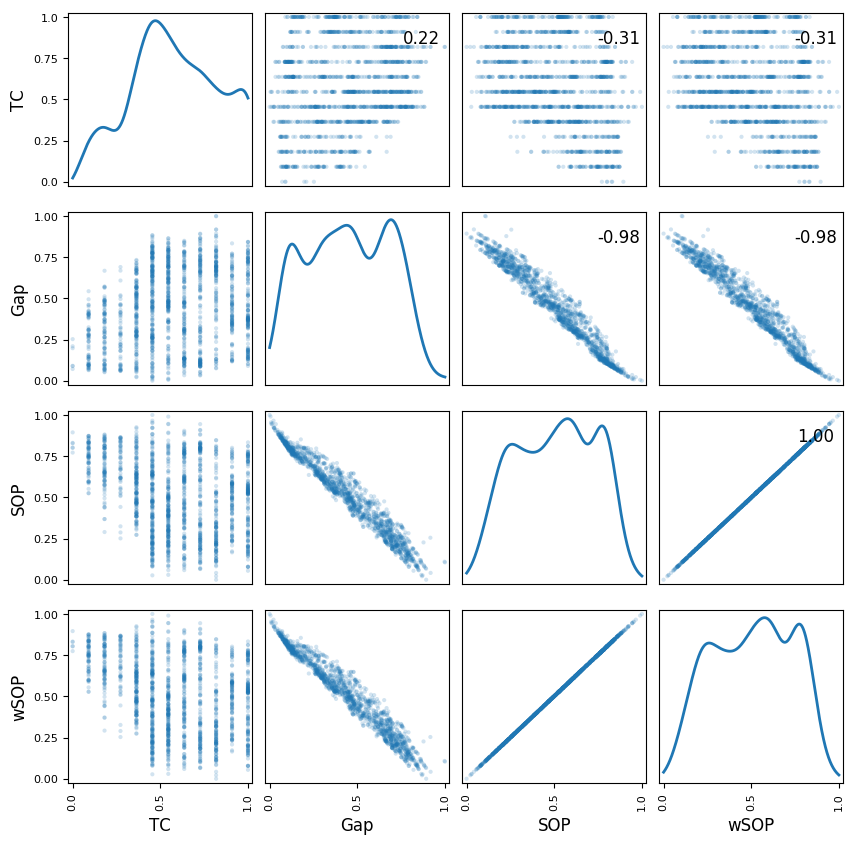
\includegraphics[width=\columnwidth]{Figure/NumGaps_SOP_TC_wSOP/precomputedInit/R4/fig/scatter_mattrix}
\caption{R4}
%\label{fig:con_pr09}
\end{subfigure}
\begin{subfigure}{0.35\textwidth}
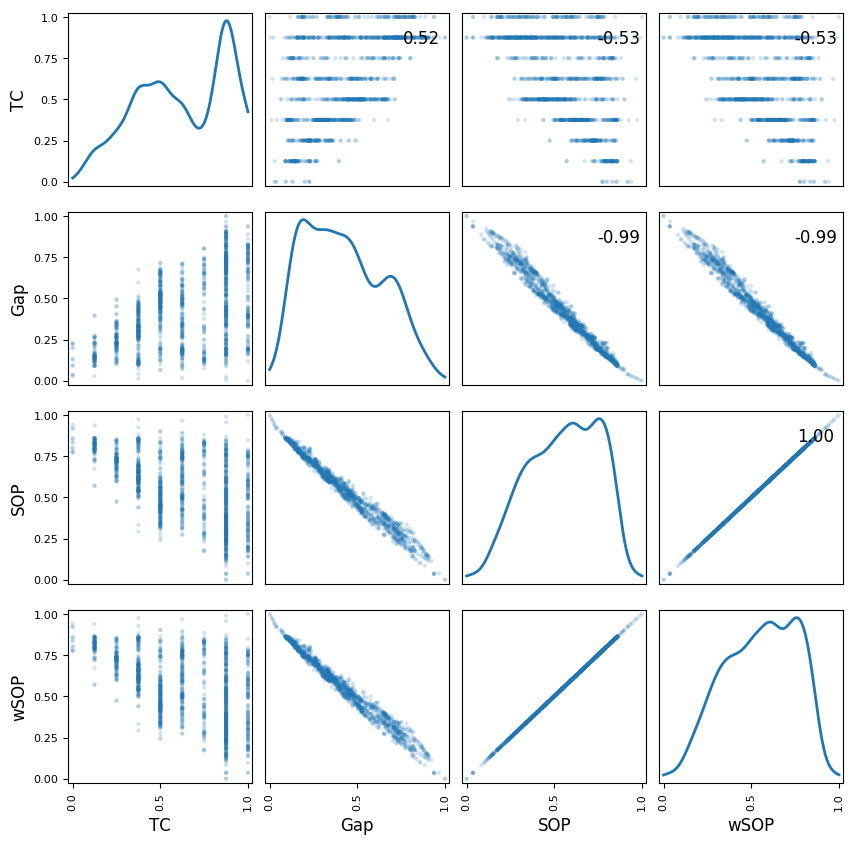
\includegraphics[width=\columnwidth]{Figure/NumGaps_SOP_TC_wSOP/precomputedInit/R9/fig/scatter_mattrix}
\caption{R9}
%\label{fig:con_pr09}
\end{subfigure}
\begin{subfigure}{0.35\textwidth}
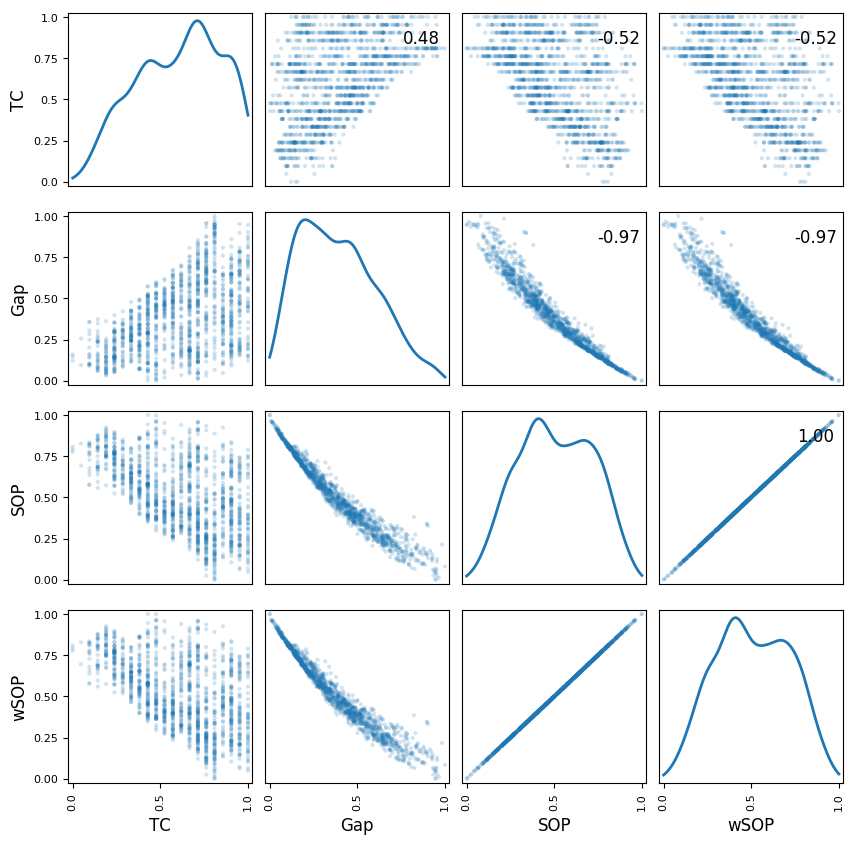
\includegraphics[width=\columnwidth]{Figure/NumGaps_SOP_TC_wSOP/precomputedInit/R14/fig/scatter_mattrix}
\caption{R14}
%\label{fig:con_pr09}
\end{subfigure}
\begin{subfigure}{0.35\textwidth}
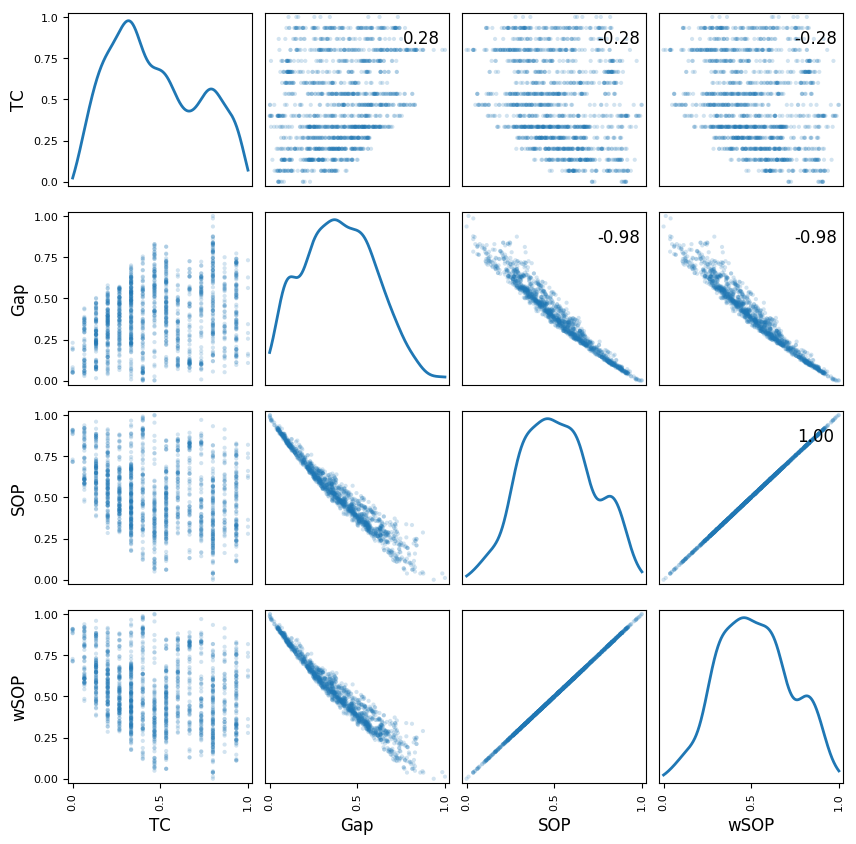
\includegraphics[width=\columnwidth]{Figure/NumGaps_SOP_TC_wSOP/precomputedInit/R19/fig/scatter_mattrix}
\caption{R19}
%\label{fig:con_pr09}
\end{subfigure}
\caption{\underline{100-taxon simulated dataset:} Scatter-plot matrices depicting the pairwise relationship of all objective functions on five randomly selected replicates. We turn each objective function into minimization form and then normalize using min-max technique. In each matrix, the diagonal cells show the distribution of objective values (estimated using KDE) while the non-diagonal cells show the correlation between pairs of objective functions. Each upper-diagonal cell contains the value of correlation coefficient $r$ of the corresponding pair of objective functions.}
\label{fig:nature_obj}
\end{adjustwidth}
\end{figure*}

\begin{figure*}[!htbp]
\centering
\small
\begin{adjustwidth}{-1cm}{-1cm}
\begin{tabular}{l||C{0.24\textwidth}|C{0.24\textwidth}|C{0.24\textwidth}|C{0.24\textwidth} }
& TC & Gap & SOP & wSOP\\\hline\hline
\rotatebox[origin=c]{-90}{R0} & 
\raisebox{-.5\height}{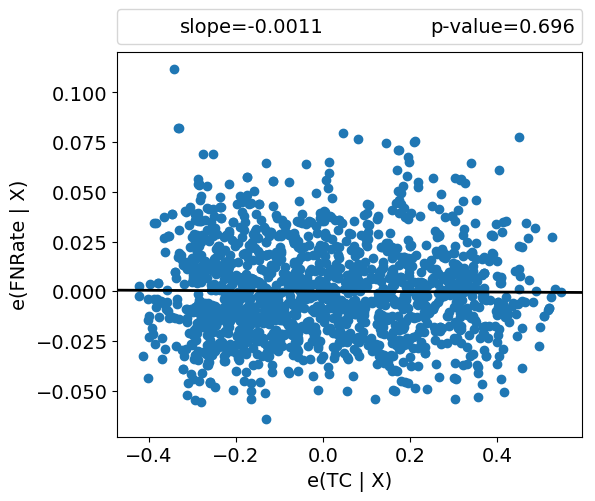
\includegraphics[width=0.25\textwidth]{Figure/NumGaps_SOP_TC_wSOP/precomputedInit/R0/fig/tc_partial_regression}} &
\raisebox{-.5\height}{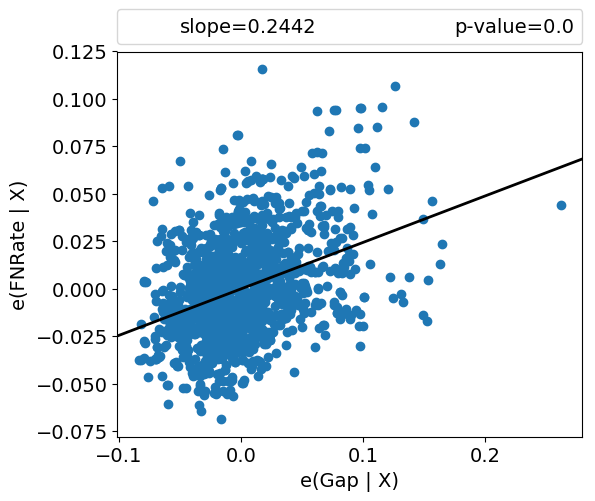
\includegraphics[width=0.25\textwidth]{Figure/NumGaps_SOP_TC_wSOP/precomputedInit/R0/fig/gap_partial_regression}} & 
\raisebox{-.5\height}{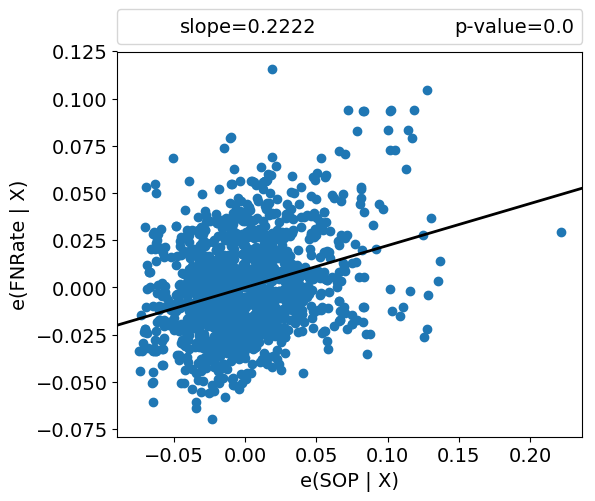
\includegraphics[width=0.25\textwidth]{Figure/NumGaps_SOP_TC_wSOP/precomputedInit/R0/fig/sop_partial_regression}} & 
\raisebox{-.5\height}{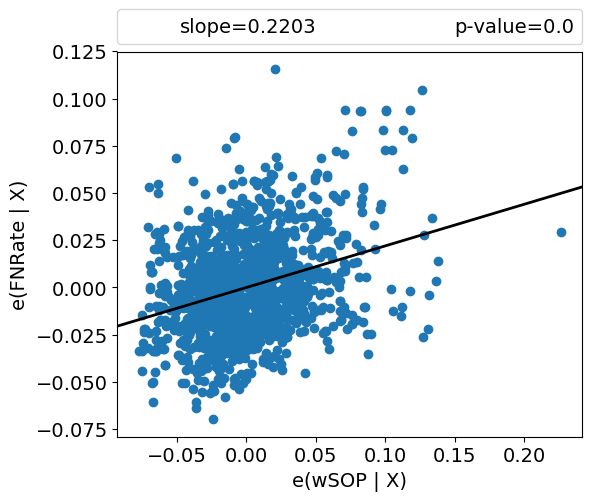
\includegraphics[width=0.25\textwidth]{Figure/NumGaps_SOP_TC_wSOP/precomputedInit/R0/fig/wsop_partial_regression}}     
\\\hline
\rotatebox[origin=c]{-90}{R4} &
\raisebox{-.5\height}{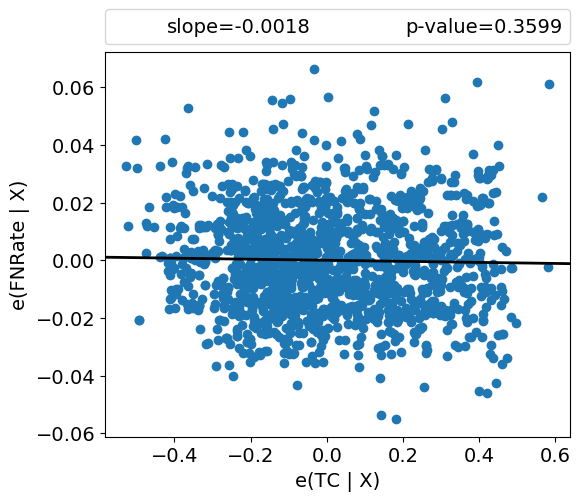
\includegraphics[width=0.25\textwidth]{Figure/NumGaps_SOP_TC_wSOP/precomputedInit/R4/fig/tc_partial_regression}} &
\raisebox{-.5\height}{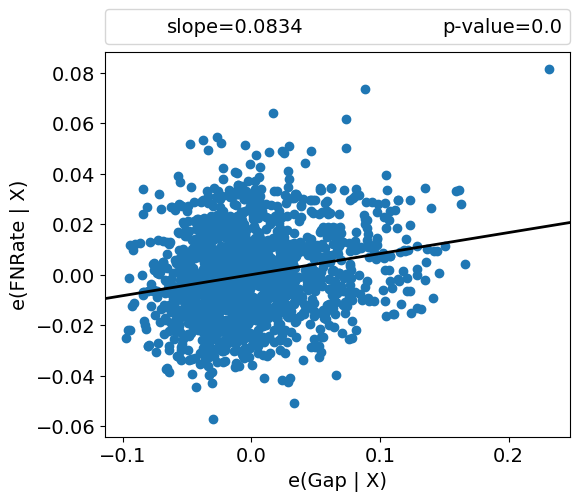
\includegraphics[width=0.25\textwidth]{Figure/NumGaps_SOP_TC_wSOP/precomputedInit/R4/fig/gap_partial_regression}} & 
\raisebox{-.5\height}{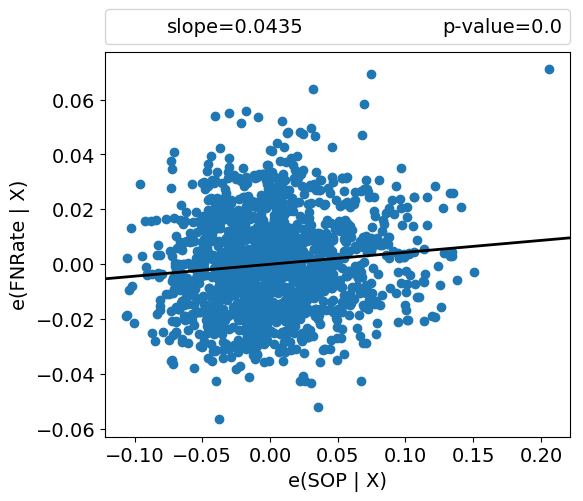
\includegraphics[width=0.25\textwidth]{Figure/NumGaps_SOP_TC_wSOP/precomputedInit/R4/fig/sop_partial_regression}} & 
\raisebox{-.5\height}{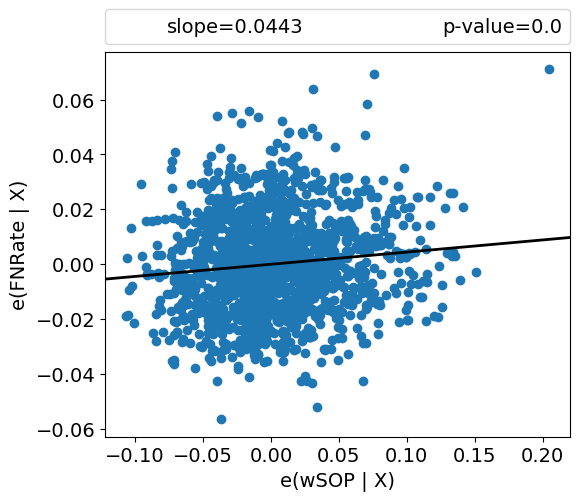
\includegraphics[width=0.25\textwidth]{Figure/NumGaps_SOP_TC_wSOP/precomputedInit/R4/fig/wsop_partial_regression}}
\\\hline
\rotatebox[origin=c]{-90}{R9} &
\raisebox{-.5\height}{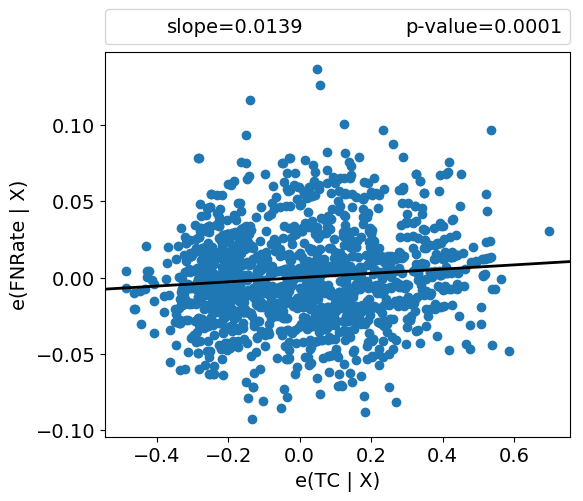
\includegraphics[width=0.25\textwidth]{Figure/NumGaps_SOP_TC_wSOP/precomputedInit/R9/fig/tc_partial_regression}} &
\raisebox{-.5\height}{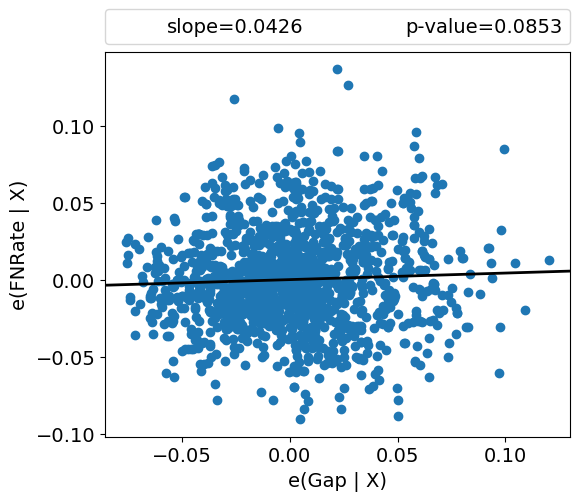
\includegraphics[width=0.25\textwidth]{Figure/NumGaps_SOP_TC_wSOP/precomputedInit/R9/fig/gap_partial_regression}} & 
\raisebox{-.5\height}{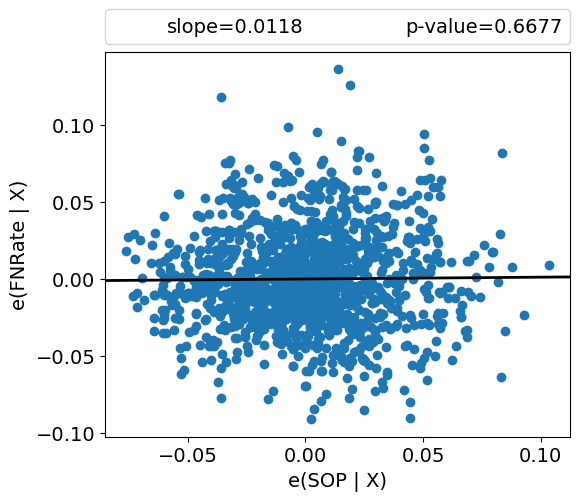
\includegraphics[width=0.25\textwidth]{Figure/NumGaps_SOP_TC_wSOP/precomputedInit/R9/fig/sop_partial_regression}} & 
\raisebox{-.5\height}{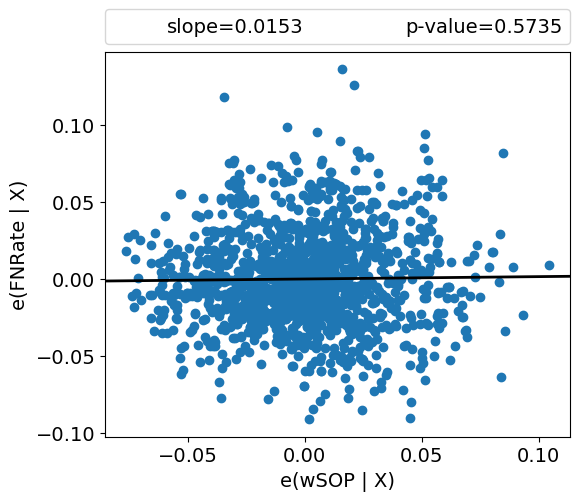
\includegraphics[width=0.25\textwidth]{Figure/NumGaps_SOP_TC_wSOP/precomputedInit/R9/fig/wsop_partial_regression}}
\\\hline
\rotatebox[origin=c]{-90}{R14} &
\raisebox{-.5\height}{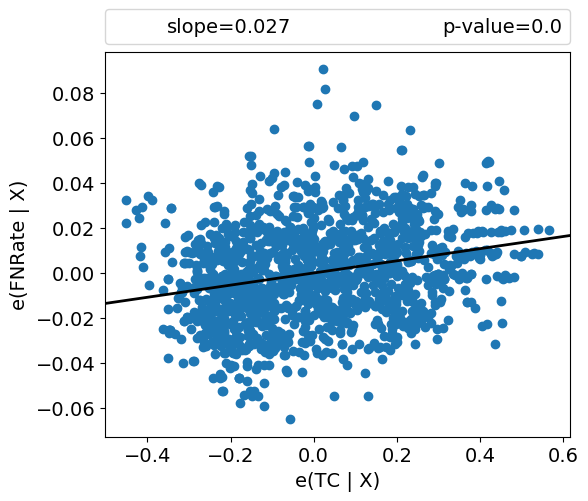
\includegraphics[width=0.25\textwidth]{Figure/NumGaps_SOP_TC_wSOP/precomputedInit/R14/fig/tc_partial_regression}} &
\raisebox{-.5\height}{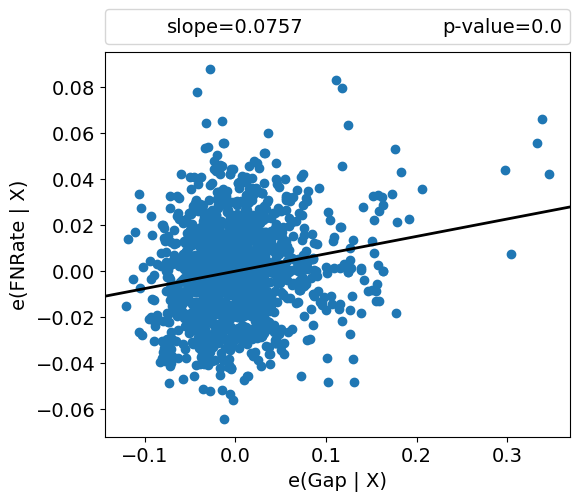
\includegraphics[width=0.25\textwidth]{Figure/NumGaps_SOP_TC_wSOP/precomputedInit/R14/fig/gap_partial_regression}} & 
\raisebox{-.5\height}{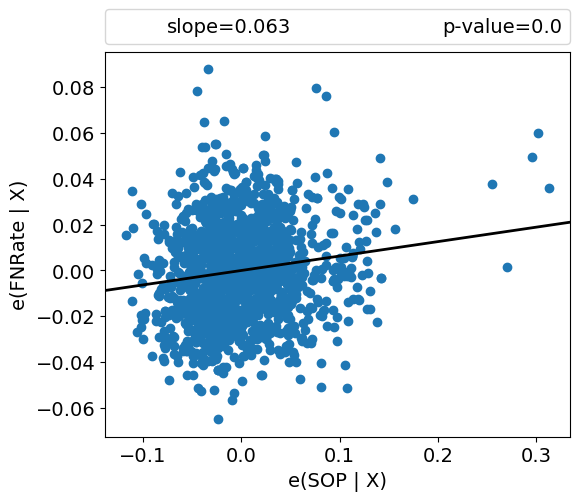
\includegraphics[width=0.25\textwidth]{Figure/NumGaps_SOP_TC_wSOP/precomputedInit/R14/fig/sop_partial_regression}} & 
\raisebox{-.5\height}{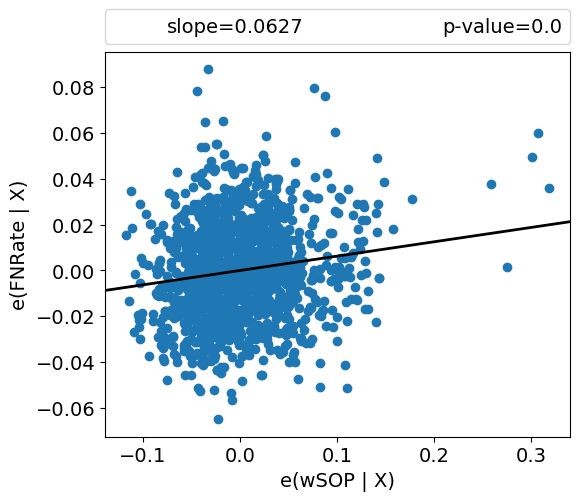
\includegraphics[width=0.25\textwidth]{Figure/NumGaps_SOP_TC_wSOP/precomputedInit/R14/fig/wsop_partial_regression}}
\\\hline
\rotatebox[origin=c]{-90}{R19} &
\raisebox{-.5\height}{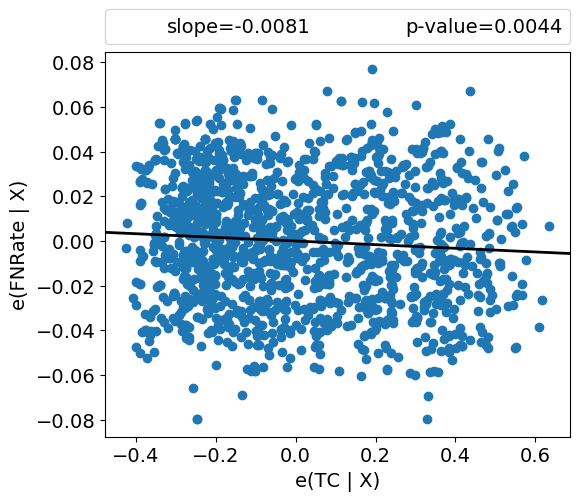
\includegraphics[width=0.25\textwidth]{Figure/NumGaps_SOP_TC_wSOP/precomputedInit/R19/fig/tc_partial_regression}} &
\raisebox{-.5\height}{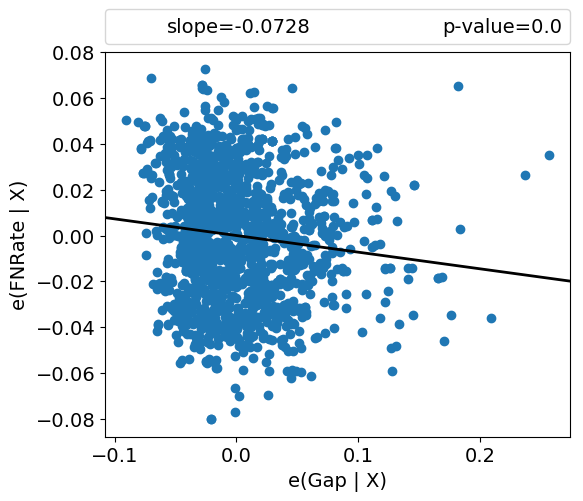
\includegraphics[width=0.25\textwidth]{Figure/NumGaps_SOP_TC_wSOP/precomputedInit/R19/fig/gap_partial_regression}} & 
\raisebox{-.5\height}{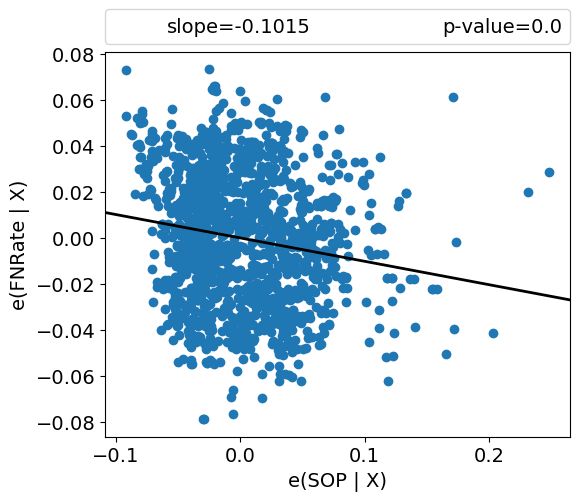
\includegraphics[width=0.25\textwidth]{Figure/NumGaps_SOP_TC_wSOP/precomputedInit/R19/fig/sop_partial_regression}} & 
\raisebox{-.5\height}{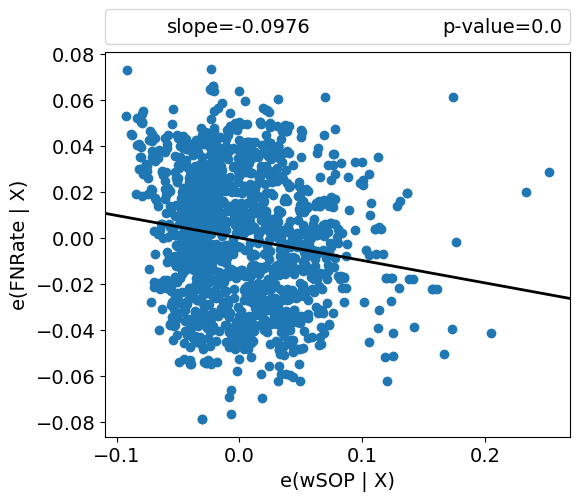
\includegraphics[width=0.25\textwidth]{Figure/NumGaps_SOP_TC_wSOP/precomputedInit/R19/fig/wsop_partial_regression}}
\\\hline
\end{tabular}
\caption{\underline{100-taxon simulated dataset:} Multiple linear regression model for identifying the association among FN rate and three objective functions (TC, Gap and SOP/wSOP) fitted to five randomly selected replicates. There is one figure for each possible combination (replicate, objective function). Each partial regression plot shows the association between an objective function and FN rate while holding the remaining two objectives constant. In a plot for an objective function $ OF $, the horizontal axis, $e(OF|X)$, denotes the residuals from regressing $OF$ against the remaining objective functions and the vertical axis, $e(FNRate|X)$, denotes the residuals from regressing FN rate against all the objective functions except $ OF $.} 
\label{fig:mul_lin_reg}
\end{adjustwidth}
\end{figure*}

\begin{figure*}[!htbp]
\centering
\begin{adjustwidth}{-1cm}{-1cm}
\begin{subfigure}{0.22\textwidth}
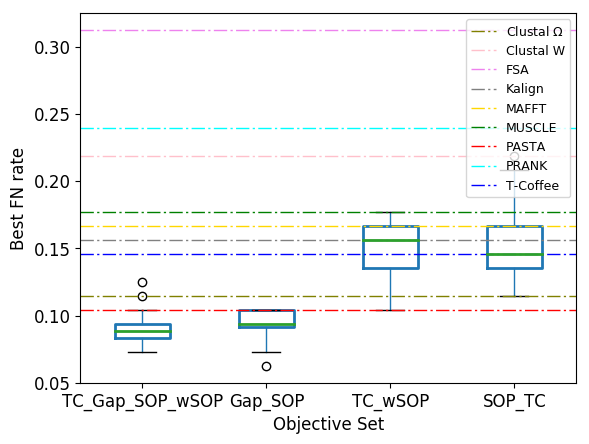
\includegraphics[width=\columnwidth]{Figure/summary/precomputedInit/R0/objset_fnrate_rank}
\caption{R0}
%\label{fig:con_pr09}
\end{subfigure}    
\begin{subfigure}{0.22\textwidth}
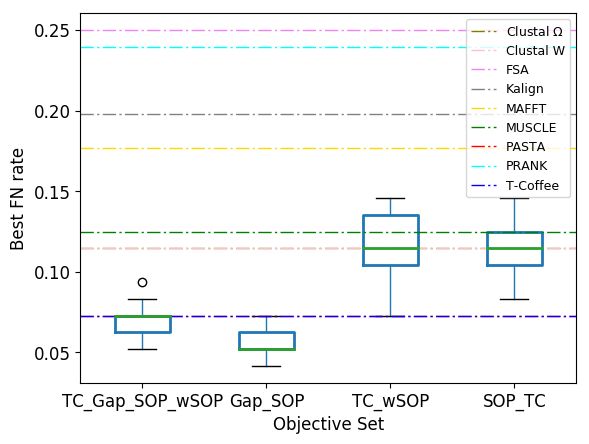
\includegraphics[width=\columnwidth]{Figure/summary/precomputedInit/R4/objset_fnrate_rank}
\caption{R4}
%\label{fig:con_pr09}
\end{subfigure}
\begin{subfigure}{0.22\textwidth}
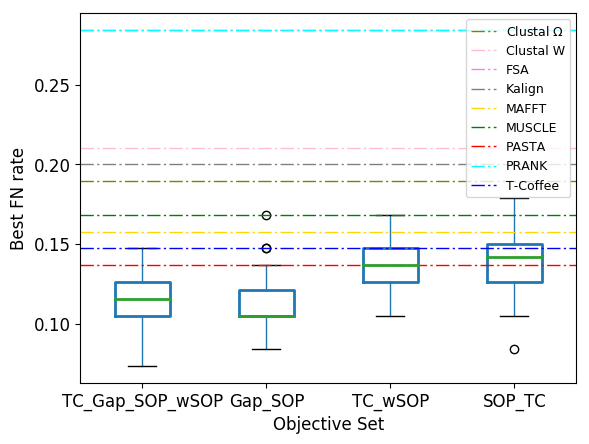
\includegraphics[width=\columnwidth]{Figure/summary/precomputedInit/R9/objset_fnrate_rank}
\caption{R9}
%\label{fig:con_pr09}
\end{subfigure}
\begin{subfigure}{0.22\textwidth}
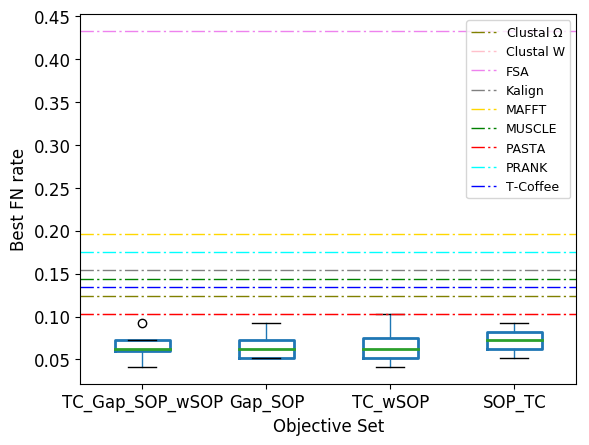
\includegraphics[width=\columnwidth]{Figure/summary/precomputedInit/R14/objset_fnrate_rank}
\caption{R14}
%\label{fig:con_pr09}
\end{subfigure}
\begin{subfigure}{0.22\textwidth}
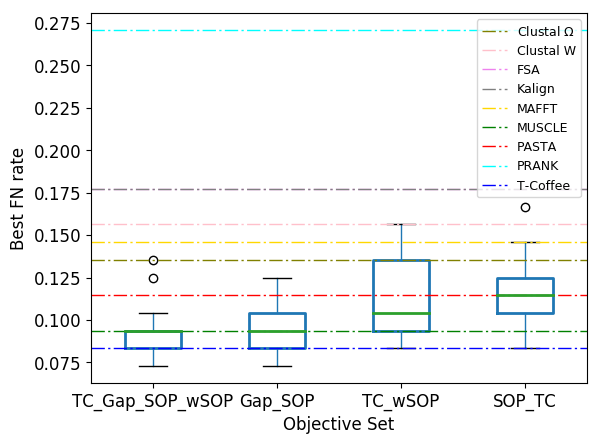
\includegraphics[width=\columnwidth]{Figure/summary/precomputedInit/R19/objset_fnrate_rank}
\caption{R19}
%\label{fig:con_pr09}
\end{subfigure}
\caption{\underline{100-taxon simulated dataset:} Comparison among objective sets based on the distribution of the collection of the best FN rates from each run. The performance of the state-of-the-art tools are shown using horizontal lines.}
\label{fig:rank_best_fn_rate}
\end{adjustwidth}
\end{figure*}
\end{comment}

\subsubsection{Selection from among the existing formulations}
\label{sec:existing_msa_formulation}
To reduce the computational effort, we pre-select three multi-objective formulations of MSA and limit our investigation thereon. Thus we choose one of the formulations from among \{Gap, SOP\}~\citep{abbasi2015local}, \{SOP, TC\}~\citep{da2010alineaga} and \{wSOP, TC\}~\citep{rubio2016hybrid} (please see Section~\ref{sec:methods} Table~\ref{tab:abbr}). We experiment with five randomly selected replicates (R0, R4, R9, R14, R19) and then judge based on two criteria: firstly, we used multiple linear regression analysis to examine the association between individual objective function and FN rate; secondly, we assess the alignments generated through the optimization of each set of objective functions in terms of resultant ML trees. 

We need to consider the relationship between each pair of objective functions to properly interpret the result of multiple linear regression. We perform this by running an appropriate multi-objective metaheuristic (i.e., NSGA-III~\citep{deb2014evolutionary}) for 25 times which simultaneously optimizes all the objective functions (i.e., \{Gap, SOP, wSOP, TC\}) and thus we obtain a large collection of diverse alignments be merging the sets of solutions output by each run. 
%We visualize the interrelations among the objective values of those solutions using a $ 4\times4 $ scatter-plot matrix~\cite{kalyanmoy2001multi} as shown in Figure~\ref{fig:nature_obj}. Here each diagonal cell of a matrix depicts the distribution of the values of an objective function estimated using Kernel Density Estimation (KDE) and the non-diagonal cells show the correlation between each pair of objective functions. As our metaheuristic algorithm tries to minimize all objective functions, we treat the maximization objective values by multiplying with -1. In the sequel, we normalize all the objective values using min-max technique and as such the maximization objectives are turned into minimization ones. 
A visualization of the interrelations among the objective values of those solutions is presented in Figure~\ref{fig:nature_obj} of the supplementary file. From these experiments, we have the following two key observations.
\begin{enumerate}[(a)]
	
	\item In all the cases, SOP is totally correlated with wSOP. So we do not need to optimize both of them. Moreover, this high correlation creates a serious problem in multiple regression analysis called multicollinearity~\citep{montgomery2012introduction}. Therefore, we should not keep these two objective functions together in our regression analysis. Also, it is redundant to consider both of them in the multi-objective formulation. 
	
	\item SOP is clearly in conflict with Gap across all the replicates. Therefore, if we optimize them simultaneously, we can generate many diverse solutions which represent the compromise between these two objective functions~\citep{kalyanmoy2001multi}. This diverse collection is likely to contain the desired alignment for any kind of dataset.
	
\end{enumerate}

As the objective functions are inter-related, we need to measure the degree of association between an objective and FN rate while holding the remaining objectives constant to avoid getting any spurious result~\citep{montgomery2012introduction}. Therefore, we perform multiple linear regression by employing the following model:
\begin{equation}
\small
\begin{split}
\text{FN rate} = \beta_0 + \beta_1 \times \text{TC}+ \beta_2 \times \text{Gap} + \\
\beta_3 \times \text{SOP (or wSOP)} + \epsilon \label{eq:multi_lin_reg}
\end{split}
\end{equation}

Each coefficient ($\beta_1, \beta_2$ and $\beta_3$) represents the expected change in the FN rate per unit change in the corresponding objective function when all the remaining objective functions are held constant. For this reason, they ($\beta_i$) are called partial regression coefficients. $\epsilon$ is the random error component which is assumed to follow a Gaussian distribution with mean zero and some fixed standard deviation. We fit this model to the solutions generated by optimizing the set \{Gap, SOP, wSOP, TC\}. For each of those solutions, we estimate the ML tree and evaluate its quality in terms of FN rate.  
%We estimate these coefficients using least-squares method and illustrate them using partial regression plots~\citep{montgomery2012introduction} in Figure~\ref{fig:mul_lin_reg}. We apply $t$-test on individual regression coefficient (i.e., slope) $\beta_i$ (with null hypothesis $\beta_i=0$) to test the significance of that association. The test results (slope, $p$-value) are incorporated in the figure. We can note the following two interesting points from these results.
We estimate these coefficients using the least-squares method (an illustration is presented in Figure~\ref{fig:mul_lin_reg} of the supplementary file). We apply $t$-test on individual regression coefficient (i.e., slope) $\beta_i$ (with null hypothesis $\beta_i=0$) to test the significance of that association. We can note the following two interesting points from these results.
\begin{enumerate}[(a)]
	\item In the majority of the cases (R0, R4 and R14), Gap, SOP and wSOP exhibit a good degree of association with FN rate (i.e positive slope) with high confidence (p-value close to 0) compared to other objective functions. So, we can expect them to be good optimization objectives for MSA.
	\item For replicate R4 and R19, none of the objective exhibit good association. This shows that an objective function might not perform well across all problem instances. 
	%\item We notice that for R19, the slope directions are opposite to our expectation. And for R19, the slope directions are opposite to our expectation.  
\end{enumerate}

Now we measure the strength of each objective set based on the FN rate achieved by the members of the generated solution set. To accomplish this, for each set of objective functions, we run a suitable multi-objective metaheuristics (NSGA-II~\citep{deb2002fast}) for 20 times following the standard practice of operations research (OR) literature (due to the stochastic nature of metaheuristics). Each run generates a set of solutions that represents the trade-offs in satisfying all objectives. Afterwards, we inferred the ML tree for each of the generated alignment. We collected the best FN rates from each of the 20 solution sets and examine the distribution of these FN rates (a visualization of these distributions using boxplots is presented in Figure~\ref{fig:rank_best_fn_rate} of the supplementary file). Here we have the following key observations:
\begin{itemize}
	\item For most of the cases, the combined set \{TC, Gap, SOP, wSOP\} achieves better results than the other sets. This indicates that adding suitable objective functions increase the chance of achieving the best FN rate. However, this can increase the overall complexity of the multi-objective metaheuristic. So in this study, we keep the size of the objective set as small as possible.
	%\item For R19, where we saw an unusual regression result, the objective sets perform worse compared to other replicates.
	\item Among our three pre-selected objective sets, \{Gap, SOP\} achieves relatively lower FN rates. This is consistent with the regression results discussed earlier.
	\item Both \{TC, Gap, SOP, wSOP\} and \{Gap, SOP\} persistently yield better FN rates than the state-of-the-art tools.
\end{itemize}
Based on our findings discussed so far, we consider \{Gap, SOP\} to be the most suitable candidate to conduct our study among all the formulations considered above. %Therefore, we run our algorithm using this set for the remaining datasets.

\begin{comment}

\begin{figure*}[!htbp]    
\begin{adjustwidth}{-1cm}{-1cm}
\centering
\begin{subfigure}{0.35\textwidth}
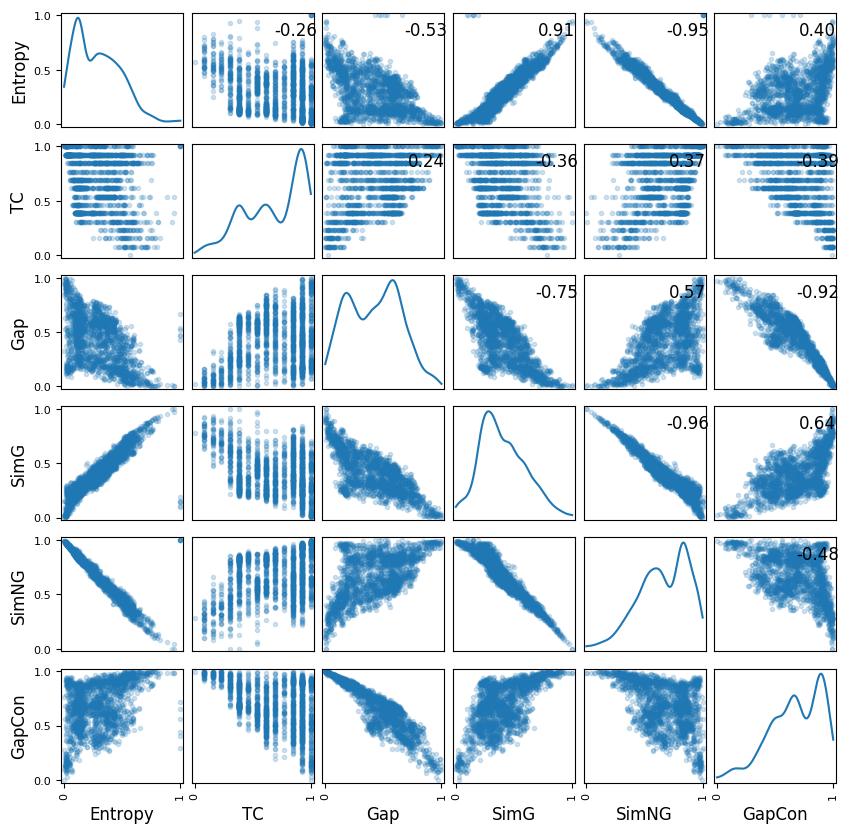
\includegraphics[width=\columnwidth]{Figure/6-obj-old/R0/fig/scatter_mattrix}
\caption{R0}
%\label{fig:con_pr09}
\end{subfigure}    
\begin{subfigure}{0.35\textwidth}
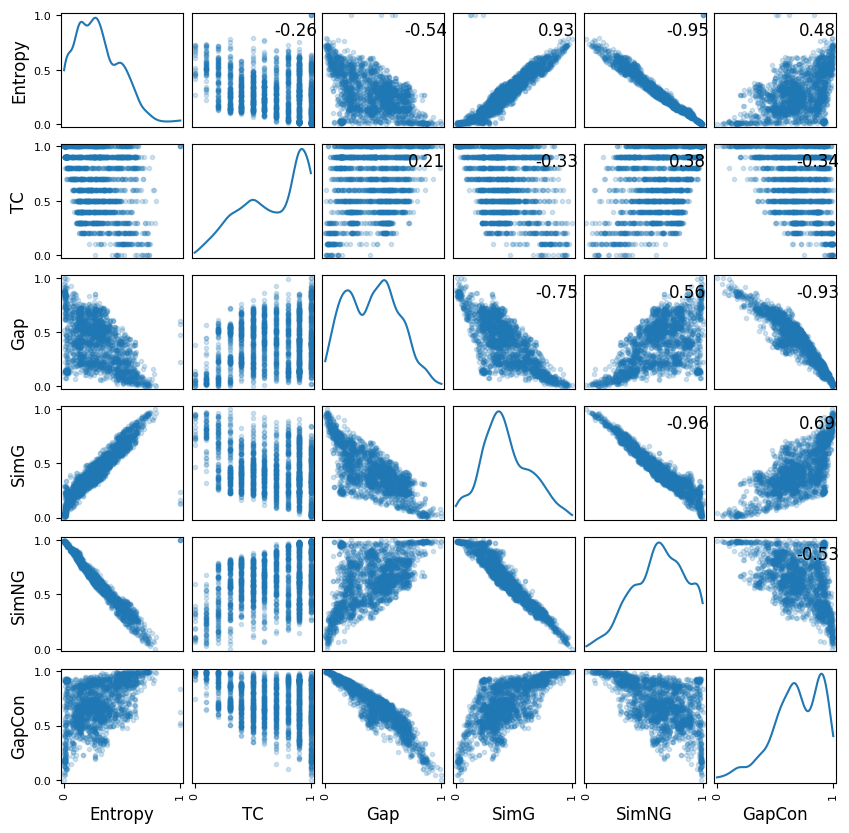
\includegraphics[width=\columnwidth]{Figure/6-obj-old/R4/fig/scatter_mattrix}
\caption{R4}
%\label{fig:con_pr09}
\end{subfigure}
\begin{subfigure}{0.35\textwidth}
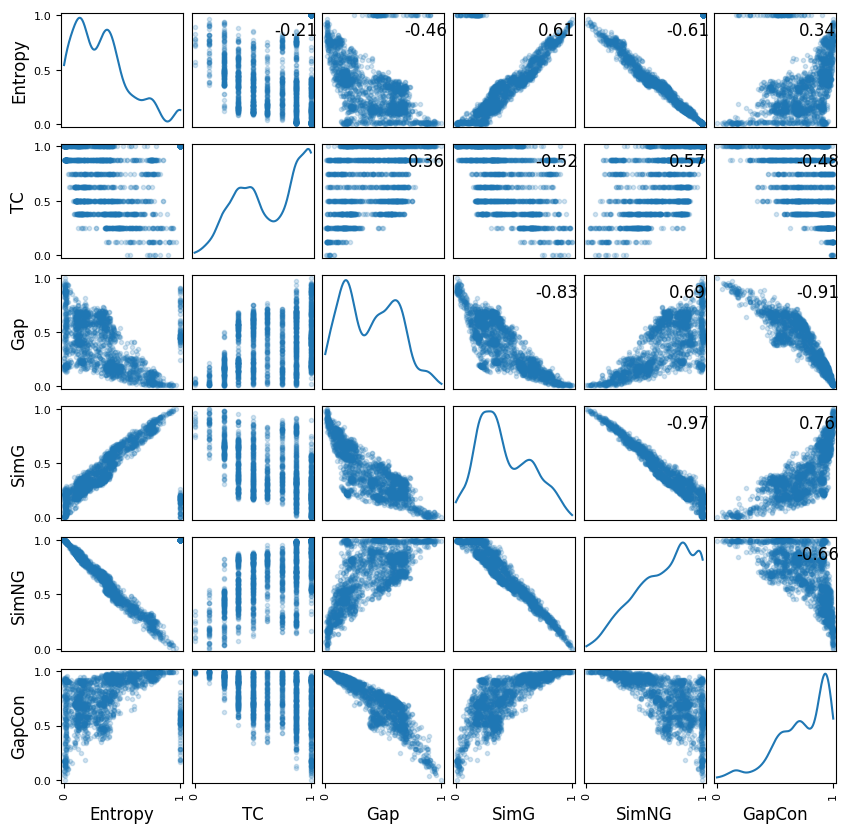
\includegraphics[width=\columnwidth]{Figure/6-obj-old/R9/fig/scatter_mattrix}
\caption{R9}
%\label{fig:con_pr09}
\end{subfigure}
\begin{subfigure}{0.35\textwidth}
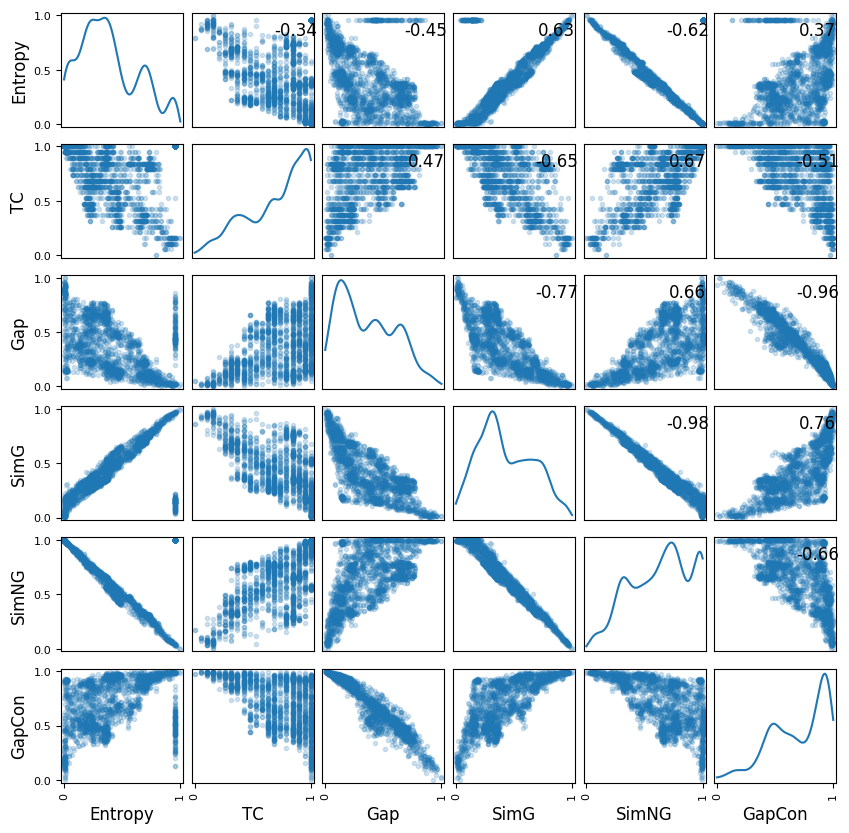
\includegraphics[width=\columnwidth]{Figure/6-obj-old/R14/fig/scatter_mattrix}
\caption{R14}
%\label{fig:con_pr09}
\end{subfigure}
\begin{subfigure}{0.35\textwidth}
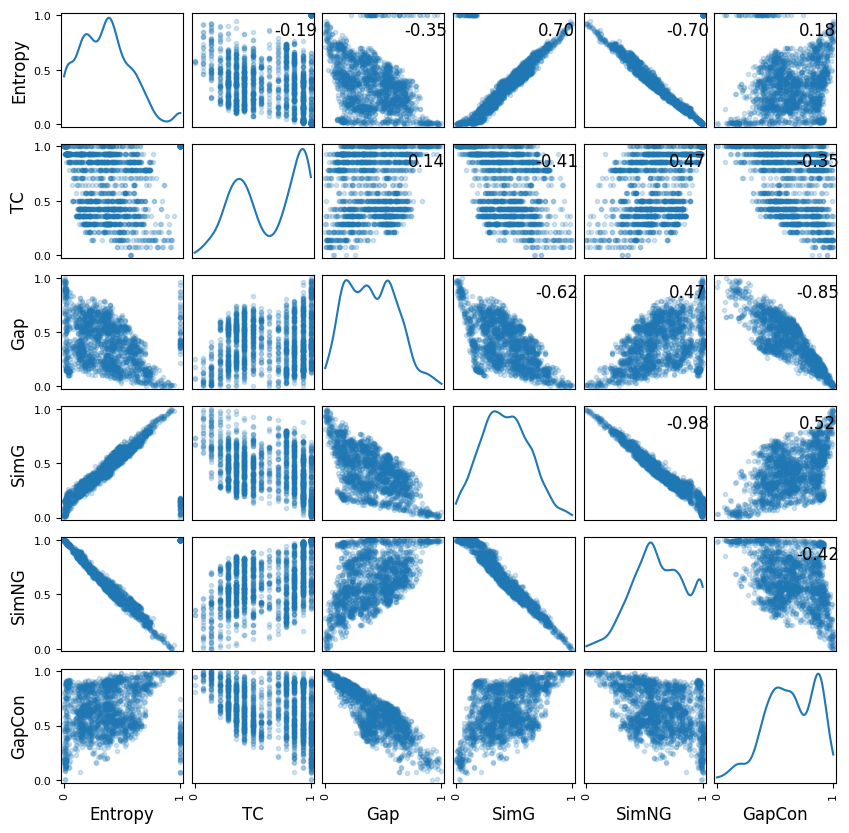
\includegraphics[width=\columnwidth]{Figure/6-obj-old/R19/fig/scatter_mattrix}
\caption{R19}
%\label{fig:con_pr09}
\end{subfigure}
\caption{\underline{100-taxon simulated dataset:} Scatter-plot matrices depicting the pairwise relationship of all objective functions on five randomly selected replicates. We turn each objective function into minimization form and then normalize using min-max technique. In each matrix, the diagonal cells show the distribution of objective values (estimated using KDE) while the non-diagonal cells show the correlation between pairs of objective functions. Each upper-diagonal cell contains the value of correlation coefficient $r$ of the corresponding pair of objective functions.}
\label{fig:new_nature_obj}
\end{adjustwidth}
\end{figure*}
\begin{figure*}[!htbp]
\centering
\small
\begin{adjustwidth}{-1cm}{-1cm}
\begin{tabular}{l||C{0.24\textwidth}|C{0.24\textwidth}|C{0.24\textwidth}|C{0.24\textwidth} }
& Entropy & GapCon & SimG & SimNG\\\hline\hline
\rotatebox[origin=c]{-90}{R0} & 
\raisebox{-.5\height}{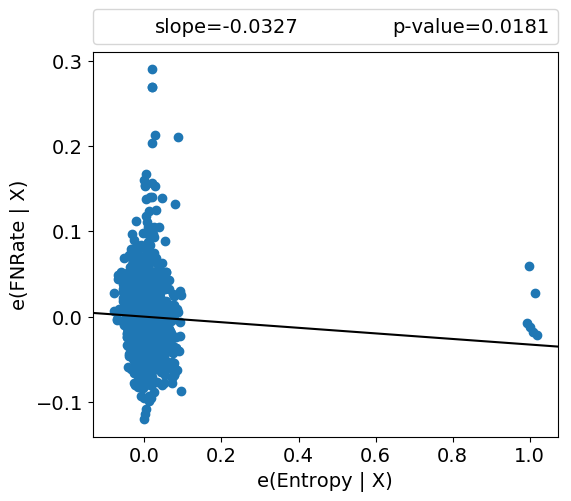
\includegraphics[width=0.25\textwidth]{Figure/6-obj-old/precomputedInit/R0/fig/Entropy_partial_regression}} &
\raisebox{-.5\height}{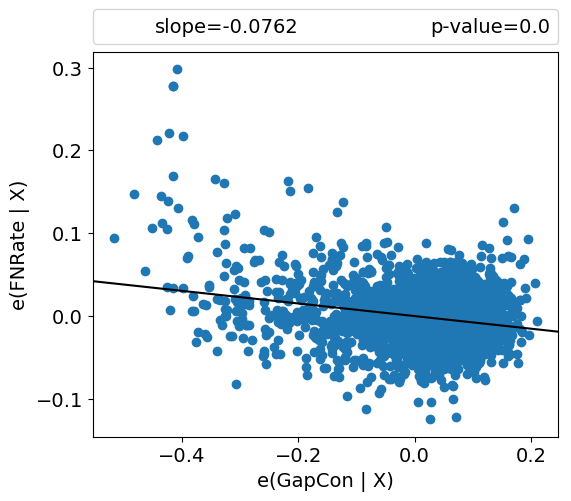
\includegraphics[width=0.25\textwidth]{Figure/6-obj-old/precomputedInit/R0/fig/GapCon_partial_regression}} & 
\raisebox{-.5\height}{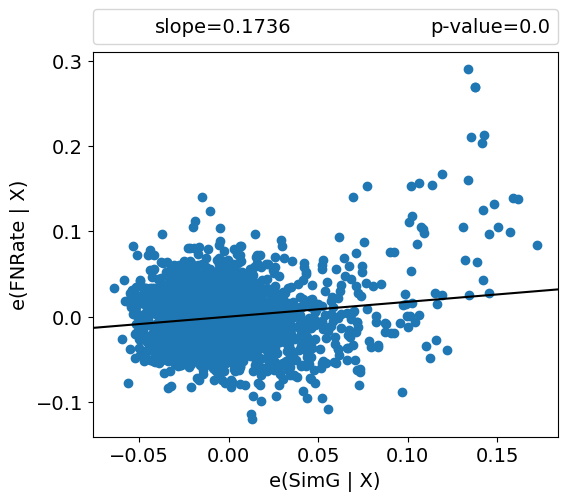
\includegraphics[width=0.25\textwidth]{Figure/6-obj-old/precomputedInit/R0/fig/SimG_partial_regression}} & 
\raisebox{-.5\height}{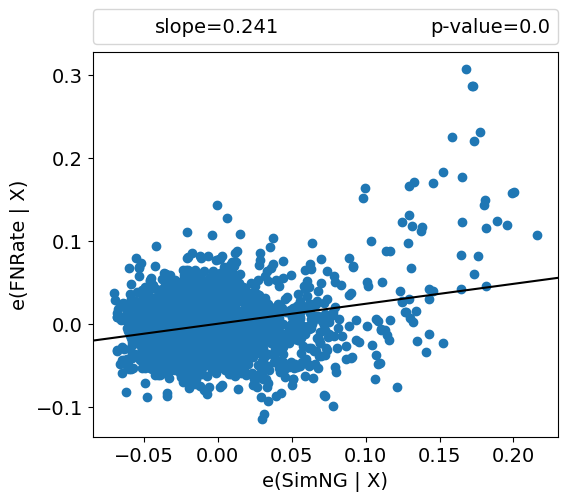
\includegraphics[width=0.25\textwidth]{Figure/6-obj-old/precomputedInit/R0/fig/SimNG_partial_regression}}     
\\\hline
\rotatebox[origin=c]{-90}{R4} &
\raisebox{-.5\height}{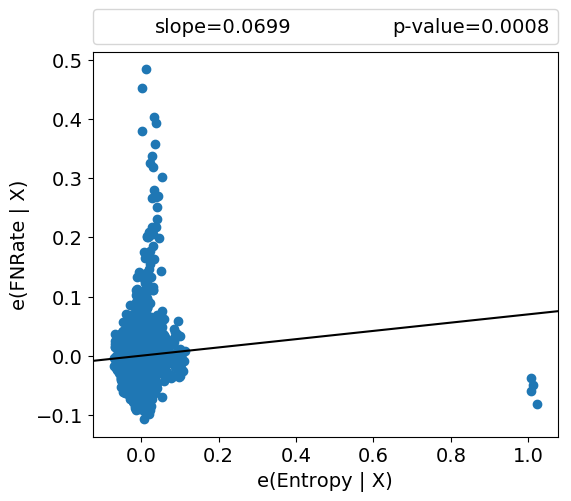
\includegraphics[width=0.25\textwidth]{Figure/6-obj-old/precomputedInit/R4/fig/Entropy_partial_regression}} &
\raisebox{-.5\height}{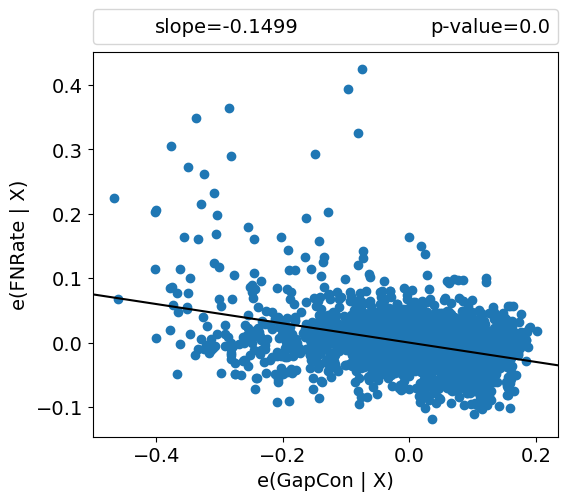
\includegraphics[width=0.25\textwidth]{Figure/6-obj-old/precomputedInit/R4/fig/GapCon_partial_regression}} & 
\raisebox{-.5\height}{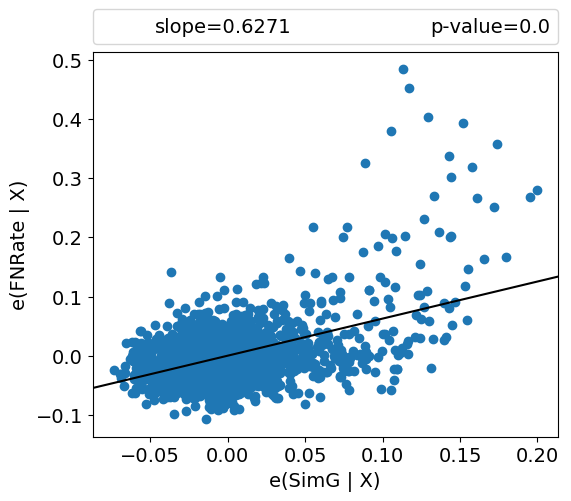
\includegraphics[width=0.25\textwidth]{Figure/6-obj-old/precomputedInit/R4/fig/SimG_partial_regression}} & 
\raisebox{-.5\height}{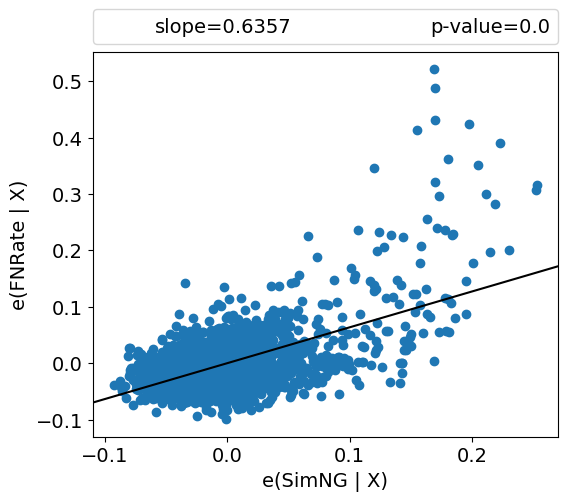
\includegraphics[width=0.25\textwidth]{Figure/6-obj-old/precomputedInit/R4/fig/SimNG_partial_regression}}
\\\hline
\rotatebox[origin=c]{-90}{R9} &
\raisebox{-.5\height}{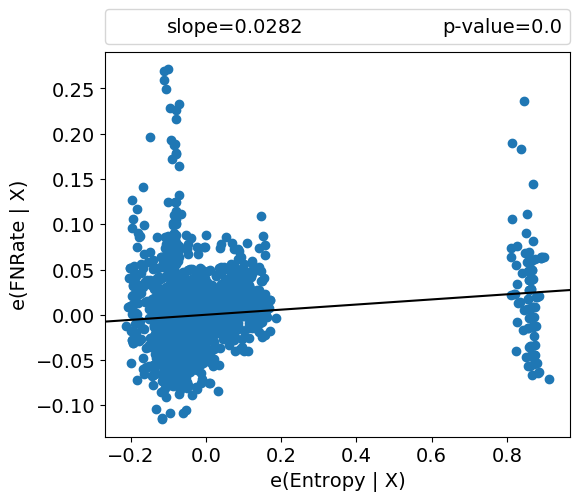
\includegraphics[width=0.25\textwidth]{Figure/6-obj-old/precomputedInit/R9/fig/Entropy_partial_regression}} &
\raisebox{-.5\height}{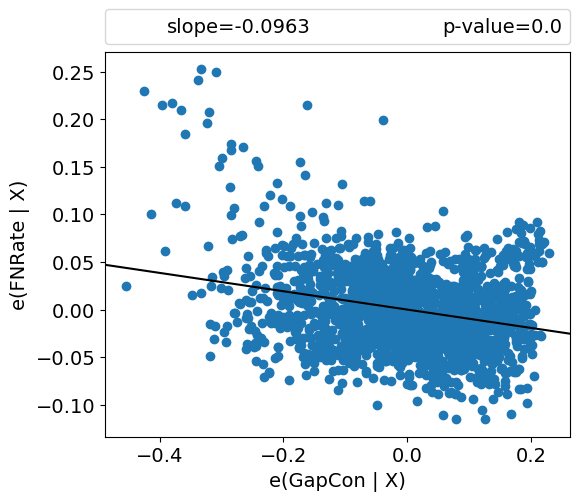
\includegraphics[width=0.25\textwidth]{Figure/6-obj-old/precomputedInit/R9/fig/GapCon_partial_regression}} & 
\raisebox{-.5\height}{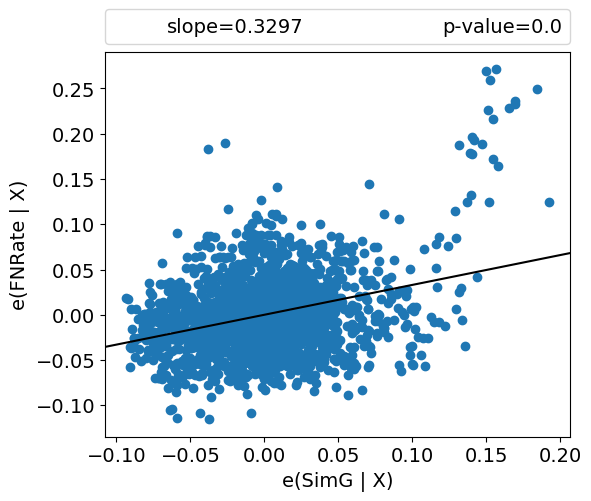
\includegraphics[width=0.25\textwidth]{Figure/6-obj-old/precomputedInit/R9/fig/SimG_partial_regression}} & 
\raisebox{-.5\height}{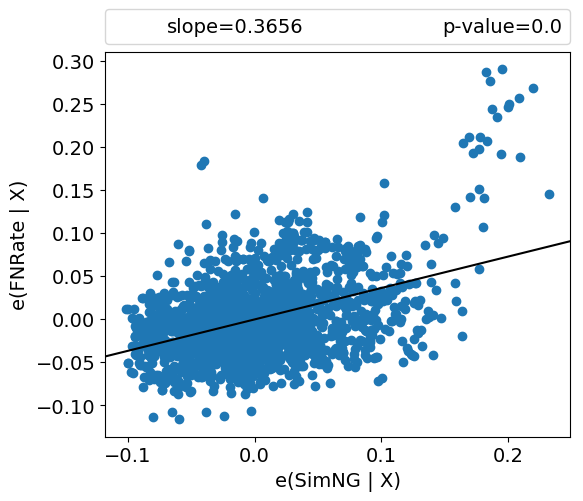
\includegraphics[width=0.25\textwidth]{Figure/6-obj-old/precomputedInit/R9/fig/SimNG_partial_regression}}
\\\hline
\rotatebox[origin=c]{-90}{R14} &
\raisebox{-.5\height}{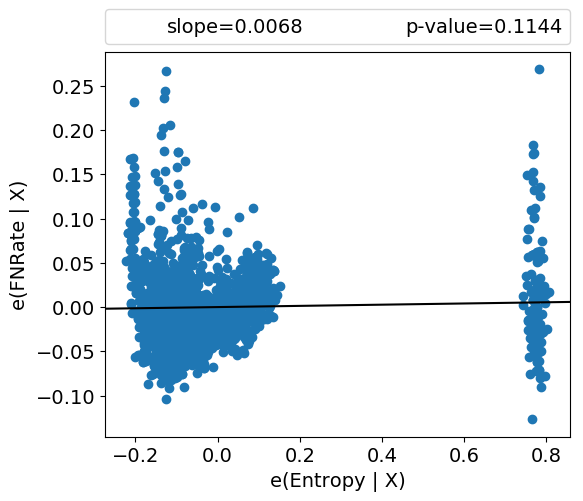
\includegraphics[width=0.25\textwidth]{Figure/6-obj-old/precomputedInit/R14/fig/Entropy_partial_regression}} &
\raisebox{-.5\height}{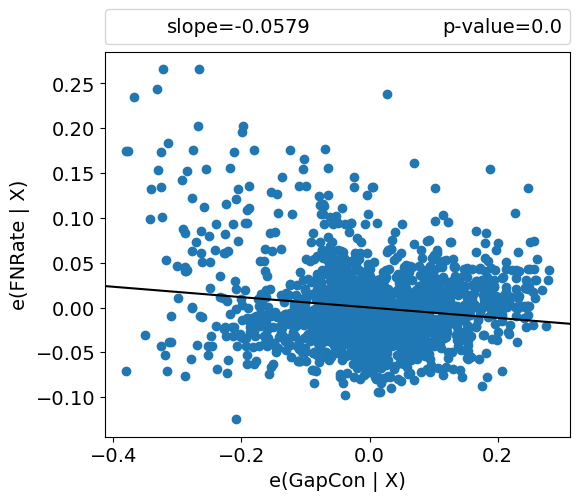
\includegraphics[width=0.25\textwidth]{Figure/6-obj-old/precomputedInit/R14/fig/GapCon_partial_regression}} & 
\raisebox{-.5\height}{\includegraphics[width=0.25\textwidth]{Figure/6-obj-old/precomputedInit/R14/fig/SimG_partial_regression}} & 
\raisebox{-.5\height}{\includegraphics[width=0.25\textwidth]{Figure/6-obj-old/precomputedInit/R14/fig/SimNG_partial_regression}}
\\\hline
\rotatebox[origin=c]{-90}{R19} &
\raisebox{-.5\height}{\includegraphics[width=0.25\textwidth]{Figure/6-obj-old/precomputedInit/R19/fig/Entropy_partial_regression}} &
\raisebox{-.5\height}{\includegraphics[width=0.25\textwidth]{Figure/6-obj-old/precomputedInit/R19/fig/GapCon_partial_regression}} & 
\raisebox{-.5\height}{\includegraphics[width=0.25\textwidth]{Figure/6-obj-old/precomputedInit/R19/fig/SimG_partial_regression}} & 
\raisebox{-.5\height}{\includegraphics[width=0.25\textwidth]{Figure/6-obj-old/precomputedInit/R19/fig/SimNG_partial_regression}}
\\\hline
\end{tabular}    
\caption{\underline{100-taxon simulated dataset:} Multiple linear regression model for identifying the association among FN rate and three objective functions (SimNG, GapCon and SimG/Entropy) fitted to five randomly selected replicates. There is one figure for each possible combination (replicate, objective function). Each partial regression plot shows the association between an objective function and FN rate while holding the remaining two objectives constant.  In a plot for an objective function $ OF $, the horizontal axis, $e(OF|X)$, denotes the residuals from regressing $OF$ against the remaining objective functions and the vertical axis, $e(FNRate|X)$, denotes the residuals from regressing FN rate against all the objective functions except $ OF $.}
\label{fig:new_mul_lin_reg}
\end{adjustwidth}
\end{figure*}
\end{comment}

\subsubsection{Selection of a new formulation}
\label{sec:new_msa_formulation}
The results reported in the last subsection suggest that the objective functions that exhibit a good association with FN rate should be more effective than the other objective functions for estimating phylogenetic trees. Based on this we make an attempt to form a new objective set as follows. We first propose four new objective functions that quantify different aspects of MSA: Entropy, SimG, SimNG and GapCon (the details are presented in Section~\ref{sec:formulation}). We combine these with TC and Gap and run NSGA-III to optimize the objective set \{Entropy, TC, Gap, SimG, SimNG, GapCon\} for 40 times to generate numerous diverse alignments. We used those to examine the association of our proposed objective functions with FN rate using multiple linear regression analysis (please refer to Figure~\ref{fig:new_nature_obj} of the supplementary file for a visualization of the relationship between the relevant pairs of objective functions within the set). The key observations of this analysis are summarized as follows: 

\begin{itemize}
	\item Entropy has a strong correlation with SimG which is problematic for multiple regression analysis. So, we should not keep these two objectives at the same time in our regression model as well as in the multi-objective formulation.
	
	\item SimG and SimNG are in conflict with each other. So by optimizing them simultaneously, a multi-objective metaheuristic can generate a large number of diverse alignments.
\end{itemize}

Now we express the relationship between FN rate and the proposed objective functions using the following model:
\begin{equation}
\small
\begin{split}
\text{FN rate} = \beta_0 + \beta_1 \times \text{SimNG}+ \beta_2 \times \text{GapCon} + \\
\beta_3 \times \text{SimG (or Entropy)} + \epsilon \label{eq:new_multi_lin_reg}
\end{split}
\end{equation}

We estimate the regression coefficients by fitting the above model to the solutions generated by optimizing the objective set \{Entropy, TC, Gap, SimG, SimNG, GapCon\}. Here we find that, in each case, both SimG and SimNG exhibit a positive correlation with FN rate. So we choose \{SimG, SimNG\} as our new objective set. For a visualization of the results using partial regression plots please refer to Figure~\ref{fig:new_mul_lin_reg} of the supplementary file.


%\clearpage
\subsection{Validation of the selected multi-objective formulations}%{Results on biological rRNA datasets}
Now we examine the effectiveness of our chosen formulations (i.e. \{Gap, SOP\} and \{SimG, SimNG\}) based on two biological datasets: two biological rRNA datasets and 27 instances of the BAliBASE 3.0 benchmark. To accomplish this we conduct several independent runs of NSGA-II on each dataset considering its stochastic nature according to the standard practice of OR literature. Then we analyze the generated solutions based on the quality of the generated alignments as well as the resultant trees.

\subsubsection{Results on biological rRNA datasets}
\begin{figure*}[!htbp]
	\centering
	\begin{adjustwidth}{-0.5cm}{-0.5cm}
		\begin{subfigure}[b]{0.25\textwidth}
			\includegraphics[width=\columnwidth]{Figure/summary/precomputedInit/23S.E/fnrate_density_single_run}
			\caption{23S.E}
			%\label{fig:con_pr09}
		\end{subfigure}    
		\begin{subfigure}[b]{0.25\textwidth}
			\includegraphics[width=\columnwidth]{Figure/summary/precomputedInit/23S.E.aa_ag/fnrate_density_single_run}
			\caption{23S.E.aa\_ag}
			%\label{fig:con_pr09}
		\end{subfigure}
		\begin{subfigure}[b]{0.25\textwidth}
			\includegraphics[width=\columnwidth]{Figure/summary/precomputedInit/23S.E/objset_fnrate_rank}
			\caption{23S.E}
			%\label{fig:con_pr09}
		\end{subfigure}    
		\begin{subfigure}[b]{0.25\textwidth}
			\includegraphics[width=\columnwidth]{Figure/summary/precomputedInit/23S.E.aa_ag/objset_fnrate_rank}
			\caption{23S.E.aa\_ag}
			%\label{fig:con_pr09}
		\end{subfigure}
		%Figure 9 starts############################
		\begin{subfigure}{0.25\textwidth}
			\includegraphics[width=\columnwidth]{Figure/summary/precomputedInit/23S.E/tc_density_single_run}
			\caption{23S.E}
			%\label{fig:con_pr09}
		\end{subfigure}    
		\begin{subfigure}{0.25\textwidth}
			\includegraphics[width=\columnwidth]{Figure/summary/precomputedInit/23S.E.aa_ag/tc_density_single_run}
			\caption{23S.E.aa\_ag}
			%\label{fig:con_pr09}
		\end{subfigure}
		\begin{subfigure}{0.25\textwidth}
			\includegraphics[width=\columnwidth]{Figure/summary/precomputedInit/23S.E/objset_tc_rank}
			\caption{23S.E}
			%\label{fig:con_pr09}
		\end{subfigure}    
		\begin{subfigure}{0.25\textwidth}
			\includegraphics[width=\columnwidth]{Figure/summary/precomputedInit/23S.E.aa_ag/objset_tc_rank}
			\caption{23S.E.aa\_ag}
			%\label{fig:con_pr09}
		\end{subfigure}
		%Figur1 10 ##################
		\begin{subfigure}{0.25\textwidth}
			\includegraphics[width=\columnwidth]{Figure/summary/precomputedInit/23S.E/pairs_density_single_run}
			\caption{23S.E}
			%\label{fig:con_pr09}
		\end{subfigure}    
		\begin{subfigure}{0.25\textwidth}
			\includegraphics[width=\columnwidth]{Figure/summary/precomputedInit/23S.E.aa_ag/pairs_density_single_run}
			\caption{23S.E.aa\_ag}
			%\label{fig:con_pr09}
		\end{subfigure}
		\begin{subfigure}{0.25\textwidth}
			\includegraphics[width=\columnwidth]{Figure/summary/precomputedInit/23S.E/objset_pairs_rank}
			\caption{23S.E}
			%\label{fig:con_pr09}
		\end{subfigure}    
		\begin{subfigure}{0.25\textwidth}
			\includegraphics[width=\columnwidth]{Figure/summary/precomputedInit/23S.E.aa_ag/objset_pairs_rank}
			\caption{23S.E.aa\_ag}
			%\label{fig:con_pr09}
		\end{subfigure}
		%Figure 11###############
		\begin{subfigure}{0.26\textwidth}
			\includegraphics[width=\columnwidth]{Figure/summary/precomputedInit/23S.E/fnrate_vs_tc}
			\caption{23S.E}
			%\label{fig:con_pr09}
		\end{subfigure}    
		\begin{subfigure}{0.26\textwidth}
			\includegraphics[width=\columnwidth]{Figure/summary/precomputedInit/23S.E.aa_ag/fnrate_vs_tc}
			\caption{23S.E.aa\_ag}
			%\label{fig:con_pr09}
		\end{subfigure}
		\begin{subfigure}{0.26\textwidth}
			\includegraphics[width=\columnwidth]{Figure/summary/precomputedInit/23S.E/fnrate_vs_sp}
			\caption{23S.E}
			%\label{fig:con_pr09}
		\end{subfigure}    
		\begin{subfigure}{0.26\textwidth}
			\includegraphics[width=\columnwidth]{Figure/summary/precomputedInit/23S.E.aa_ag/fnrate_vs_sp}
			\caption{23S.E.aa\_ag}
			%\label{fig:con_pr09}
		\end{subfigure}
	
	\caption{\underline{Biological rRNA datasets:} \textbf{Panel 1 (Top Panel):} part (a) and part (b) show the averaged FN rate of 100 solutions over 10 independent runs. 
		%Since each run generates 100 solutions, we make the average meaningful by sorting the 100 FN rates per run. Then we average the best FN rates obtained across all the runs. The same applies to the second best ones and so on. 
		part (c) and part (d) show the variation of the best FN rates obtained across 10 runs using boxplots.  %In all figures, we show the performance of nine state-of-the-art tools using dashed horizontal lines.
		\textbf{Panel 2 (Panel 3):} part (e) and part (f) (part (i) and part (j)) show the TC score (SP score) of 100  solutions averaged over 10 runs. 
		%At first, we sort the TC scores (SP scores) of each solution set. Then we average the TC scores (SP score) at each sorted position of all the sets. 
		part (g) and part (h) (part (k) and part (l)) show the distribution of the best TC scores (SP scores) collected from all runs.
		%Panel 2: part (e) and part (f) show the TC score of 100  solutions averaged over 10 runs. At first, we sort the TC scores of each solution set. Then we average the TC scores at each sorted position of all the sets. part (g) and part (h) show the distribution of the best TC scores collected from all runs.\\ 
		%In each figure, The horizontal lines show the performance of the state-of-the-art tools.
		%Panel 3: part (i) and part (j) show the SP score of 100 solutions averaged over 10 runs. At first, we sort the SP scores of each solution set. Then we average the SP scores at each sorted position of all the sets. part (k) and part (l) show the distribution of the best SP scores collected from all runs.\\ 
		%In each figure, The horizontal lines show the performance of the state-of-the-art tools.
		\textbf{Panel 4 (Bottom panel):} part (m) and part (n) show the relationship between FN rate and TC score for different alignments. part (o) and part (p) show the relationship between FN rate and SP score. In all panels except for the bottom one, we show the performance of nine state-of-the-art tools using dashed horizontal lines; the horizontal lines at the bottom panel mark the FN rates achieved by those tools.
	}
	\label{fig:fn_rate_tc_sp_bio}
\end{adjustwidth}
\end{figure*}


We conducted 10 runs of NSGA-II with our two selected objective sets for two datasets, namely, 23S.E and 23S.E.aa\_ag. 
We compare the performance of the multi-objective formulations with respect to FN rate against the nine state-of-the-art tools from two perspectives in the top panel of Figure~\ref{fig:fn_rate_tc_sp_bio}. Here, part (a) and (b) show the averaged FN rate of 100 solutions over 10 runs. Since each run generates 100 solutions, we make the average meaningful by sorting the 100 FN rates per run. Then we average the best FN rates across all the runs. The same applies to the second best ones and so on. These figures (part (a) and (b)) demonstrate a promising aspect of multi-objective approach that for each data it can generate a substantial number of solutions that are better than the outputs of state-of-the-art tools. However, a practitioner would be interested in the best solutions. Therefore, we summarize the variation of the best FN rate (among 100 values) across 10 runs in part (c) and (d). We see that, for both of the datasets, FSA yielded the best performance among the nine tools, followed by PRANK for 23.S.E and PASTA for 23S.E.aa\_ag. The two multi-objective formulations helped to achieve better FN rates than FSA for 23S.E.aa\_ag (part (b) and (d)). Here, on average, \{Gap ,SOP\} generates around 10\% solutions that are better than FSA and 40\% solutions that are better than PASTA as shown in part (b). On the other hand, on average \{SimG, SimNG\} produces very few solutions that are better than FSA but around 40\% solutions that are better than PASTA. Part (d) shows that \{Gap, SOP\} consistently outperforms the best tool (FSA) whereas \{SimG, SimNG\} outperforms FSA in nearly 40\% of the total runs. Now let us see the results for 23S.E (part (a) and (c)), where both of the objective sets remain between the best (FSA) and second best (PRANK) tool. Both of them generates around 5\% solutions better than PRANK.
%and achieves around 30\% improvement compared to FSA.
%We visualize the distribution of the best FN rates collected from each run using boxplots in Figure~\ref{fig:fn_rate_bio}. In that figure, we also show the FN rates of 100 solutions. We see that for 23S.E.aa\_ag, both of the sets achieved FN rates better than the best tool FSA but \{Gap ,SOP\} is more consistent in generating good results. On the other hand, for 23S.E both the sets perform between the first and second best tool which is FSA and PRANK respectively. Here \{SimG, SimNG\} performs consistently better than the other.

We perform similar analysis based on the widely used two alignment quality measures, namely, TC score and SP score and report the results in Panel 2 and 3 of Figure~\ref{fig:fn_rate_tc_sp_bio} respectively. We notice that, according to these two popular measures, for both the datasets, the alignments generated by multi-objective formulations failed to beat the best performing tool, PASTA. The clear disagreement between FN rate and TC score (part (m) and (n)) as well as between FN rate and SP score (part (o) and (p)) has been illustrated in Panel 4 of Figure~\ref{fig:fn_rate_tc_sp_bio}. To summarize, from the analysis presented in Panel 4 (bottom panel), we realize that the tools/approaches achieving better performance than our multi-objective formulations in terms of the popular measures, namely, TC score and SP score fail to achieve better FN rates than our multi-objective formulations. To elaborate, according to TC score, PASTA is the best performer among the nine tools, and our objective sets have generated several alignments having worse (lower) TC score than PASTA (and FSA). However, those alignments can produce phylogenetic trees with better FN rates than those tools. Even from among the tools, there is disagreement between TC score and FN rate: PASTA is in fact behind FSA in terms of the latter. Similarly in part (o) and (p) of Panel 4 which is dedicated to the comparison between FN rate and SP score, we find several alignments generated by the multi-objective formulations that are worse than PASTA in terms of SP score, but, achieve better FN rates than that tool. 

%In Figure~\ref{fig:tc_bio}, we show similar results as above but based on the widely used alignment quality measure TC score. We notice that according to TC, the multi-objective formulations can hardly outperform the best tool PASTA for both of the datasets. However, interestingly our multi-objective formulations produced better phylogenetic trees. Therefore, the tool which produces better TC score does not necessarily produce better FN rate which is unexpected. We illustrate this disagreement between FN rate and TC score in the top panel of Figure~\ref{fig:fnrate_vs_tc_bio} where we plot the FN rate and TC score of the tools as well as best alignments generated by each objective set. We see that according to TC score, PASTA is the best tool while FSA performs the best based on FN rate. Moreover, our objective sets generated several alignments having worse (lower) TC score than PASTA and FSA. However, those alignments can produce phylogenetic trees with better FN rate than those tools.

%Finally, we perform similar analysis based on SP score as shown in Figure~\ref{fig:sp_bio}. Again, here we find a similar disagreement between SP score and FN rate. For both the datasets, the alignments generated by the objective sets failed to beat the best tool PASTA according to SP score. We illustrate this phenomenon in the bottom panel of Figure~\ref{fig:fnrate_vs_tc_bio}, where we find several alignments (generated by the multi-objective formulations) worse than PASTA (the best tool w.r.t. SP-score) achieve better FN rates than that tool.  


%\begin{comment}

%############################# RV11
\begin{figure*}[!htbp]
	\begin{adjustwidth}{-1cm}{-1cm}
		\centering
		\begin{subfigure}[b]{0.26\textwidth}
			\includegraphics[width=\columnwidth]{Figure/summary/precomputedInit/Balibase/BB11005_fnrate_density_single_run}
			\caption{BB11005}
			%\label{fig:con_pr09}
		\end{subfigure}    
		\begin{subfigure}[b]{0.26\textwidth}
			\includegraphics[width=\columnwidth]{Figure/summary/precomputedInit/Balibase/BB11018_fnrate_density_single_run}
			\caption{BB11018}
			%\label{fig:con_pr09}
		\end{subfigure}
		\begin{subfigure}[b]{0.26\textwidth}
			\includegraphics[width=\columnwidth]{Figure/summary/precomputedInit/Balibase/BB11020_fnrate_density_single_run}
			\caption{BB11020}
			%\label{fig:con_pr09}
		\end{subfigure}
		\begin{subfigure}[b]{0.26\textwidth}
			\includegraphics[width=\columnwidth]{Figure/summary/precomputedInit/Balibase/BB11033_fnrate_density_single_run}
			\caption{BB11033}
			%\label{fig:con_pr09}
		\end{subfigure}
		%    \begin{subfigure}{0.26\textwidth}
		%        \includegraphics[width=\columnwidth]{Figure/summary/precomputedInit/Balibase/BB11038_fnrate_density_single_run}
		%        \caption{BB11038}
		%        %\label{fig:con_pr09}
		%    \end{subfigure}
		\begin{subfigure}{0.26\textwidth}
			\includegraphics[width=\columnwidth]{Figure/summary/precomputedInit/Balibase/BB11005_objset_fnrate_rank}
			\caption{BB11005}
			%\label{fig:con_pr09}
		\end{subfigure}    
		\begin{subfigure}{0.26\textwidth}
			\includegraphics[width=\columnwidth]{Figure/summary/precomputedInit/Balibase/BB11018_objset_fnrate_rank}
			\caption{BB11018}
			%\label{fig:con_pr09}
		\end{subfigure}
		\begin{subfigure}{0.26\textwidth}
			\includegraphics[width=\columnwidth]{Figure/summary/precomputedInit/Balibase/BB11020_objset_fnrate_rank}
			\caption{BB11020}
			%\label{fig:con_pr09}
		\end{subfigure}
		%        \begin{subfigure}{0.26\textwidth}
		%            \includegraphics[width=\columnwidth]{Figure/summary/precomputedInit/Balibase/BB11029_objset_fnrate_rank}
		%            \caption{BB11029}
		%            %\label{fig:con_pr09}
		%        \end{subfigure}
		\begin{subfigure}{0.26\textwidth}
			\includegraphics[width=\columnwidth]{Figure/summary/precomputedInit/Balibase/BB11033_objset_fnrate_rank}
			\caption{BB11033}
			%\label{fig:con_pr09}
		\end{subfigure}
		
		%Fig 15
		\begin{subfigure}{0.26\textwidth}
			\includegraphics[width=\columnwidth]{Figure/summary/precomputedInit/Balibase/BB11005_fnrate_vs_tc_2}
			\caption{BB11005}
			%\label{fig:con_pr09}
		\end{subfigure}    
		\begin{subfigure}{0.26\textwidth}
			\includegraphics[width=\columnwidth]{Figure/summary/precomputedInit/Balibase/BB11018_fnrate_vs_tc_2}
			\caption{BB11018}
			%\label{fig:con_pr09}
		\end{subfigure}
		\begin{subfigure}{0.26\textwidth}
			\includegraphics[width=\columnwidth]{Figure/summary/precomputedInit/Balibase/BB11020_fnrate_vs_tc_2}
			\caption{BB11020}
			%\label{fig:con_pr09}
		\end{subfigure}
		\begin{subfigure}{0.26\textwidth}
			\includegraphics[width=\columnwidth]{Figure/summary/precomputedInit/Balibase/BB11033_fnrate_vs_tc_2}
			\caption{BB11033}
			%\label{fig:con_pr09}
		\end{subfigure}    
		\begin{subfigure}{0.26\textwidth}
			\includegraphics[width=\columnwidth]{Figure/summary/precomputedInit/Balibase/BB11005_fnrate_vs_sp_2}
			\caption{BB11005}
			%\label{fig:con_pr09}
		\end{subfigure}    
		\begin{subfigure}{0.26\textwidth}
			\includegraphics[width=\columnwidth]{Figure/summary/precomputedInit/Balibase/BB11018_fnrate_vs_sp_2}
			\caption{BB11018}
			%\label{fig:con_pr09}
		\end{subfigure}
		\begin{subfigure}{0.26\textwidth}
			\includegraphics[width=\columnwidth]{Figure/summary/precomputedInit/Balibase/BB11020_fnrate_vs_sp_2}
			\caption{BB11020}
			%\label{fig:con_pr09}
		\end{subfigure}
		\begin{subfigure}{0.26\textwidth}
			\includegraphics[width=\columnwidth]{Figure/summary/precomputedInit/Balibase/BB11033_fnrate_vs_sp_2}
			\caption{BB11033}
			%\label{fig:con_pr09}
		\end{subfigure}
	
	\caption{ \underline{RV11:} \textbf{Panel 1 (Top panel):} part (a) - (d) show the FN rate of 100 solutions averaged over 20 independent runs. 
	%At first, we sort the FN rates of each solution set. Then we average the FN rates at each sorted position of all the sets. 
	\textbf{Panel 2:} part (e) - (h) show the distribution of the best FN rates collected from all runs. 
	\textbf{Panel 3 (Panel 4):} part (i) - (l) (part (m) - (p)) show the relationship between FN rate and TC score (SP score) for different alignments. In all panels, we show the FN rates achieved by the nine state-of-the-art tools using dashed horizontal lines.}
	\label{fig:rv11_fn_rate_tc_sp}
\end{adjustwidth}
\end{figure*}


\begin{figure*}[!htbp]
	\begin{adjustwidth}{-1cm}{-1cm}
		\centering
		\begin{subfigure}[b]{0.26\textwidth}
			\includegraphics[width=\columnwidth]{Figure/summary/precomputedInit/Balibase/BB11005_tc_density_single_run_2}
			\caption{BB11005}
			%\label{fig:con_pr09}
		\end{subfigure}    
		\begin{subfigure}[b]{0.26\textwidth}
			\includegraphics[width=\columnwidth]{Figure/summary/precomputedInit/Balibase/BB11018_tc_density_single_run_2}
			\caption{BB11018}
			%\label{fig:con_pr09}
		\end{subfigure}
		\begin{subfigure}[b]{0.26\textwidth}
			\includegraphics[width=\columnwidth]{Figure/summary/precomputedInit/Balibase/BB11020_tc_density_single_run_2}
			\caption{BB11020}
			%\label{fig:con_pr09}
		\end{subfigure}
		%        \begin{subfigure}{0.22\textwidth}
		%            \includegraphics[width=\columnwidth]{Figure/summary/precomputedInit/Balibase/BB11029_tc_density_single_run_2}
		%            \caption{BB11029}
		%            %\label{fig:con_pr09}
		%        \end{subfigure}
		\begin{subfigure}[b]{0.26\textwidth}
			\includegraphics[width=\columnwidth]{Figure/summary/precomputedInit/Balibase/BB11033_tc_density_single_run_2}
			\caption{BB11033}
			%\label{fig:con_pr09}
		\end{subfigure}
		\begin{subfigure}{0.26\textwidth}
			\includegraphics[width=\columnwidth]{Figure/summary/precomputedInit/Balibase/BB11005_objset_tc_rank_2}
			\caption{BB11005}
			%\label{fig:con_pr09}
		\end{subfigure}    
		\begin{subfigure}{0.26\textwidth}
			\includegraphics[width=\columnwidth]{Figure/summary/precomputedInit/Balibase/BB11018_objset_tc_rank_2}
			\caption{BB11018}
			%\label{fig:con_pr09}
		\end{subfigure}
		\begin{subfigure}{0.26\textwidth}
			\includegraphics[width=\columnwidth]{Figure/summary/precomputedInit/Balibase/BB11020_objset_tc_rank_2}
			\caption{BB11020}
			%\label{fig:con_pr09}
		\end{subfigure}
		%        \begin{subfigure}{0.22\textwidth}
		%            \includegraphics[width=\columnwidth]{Figure/summary/precomputedInit/Balibase/BB11029_objset_tc_rank_2}
		%            \caption{BB11029}
		%            %\label{fig:con_pr09}
		%        \end{subfigure}
		\begin{subfigure}{0.26\textwidth}
			\includegraphics[width=\columnwidth]{Figure/summary/precomputedInit/Balibase/BB11033_objset_tc_rank_2}
			\caption{BB11033}
			%\label{fig:con_pr09}
		\end{subfigure}
		
		%Fig 14
		\begin{subfigure}{0.26\textwidth}
			\includegraphics[width=\columnwidth]{Figure/summary/precomputedInit/Balibase/BB11005_pairs_density_single_run_2}
			\caption{BB11005}
			%\label{fig:con_pr09}
		\end{subfigure}    
		\begin{subfigure}{0.26\textwidth}
			\includegraphics[width=\columnwidth]{Figure/summary/precomputedInit/Balibase/BB11018_pairs_density_single_run_2}
			\caption{BB11018}
			%\label{fig:con_pr09}
		\end{subfigure}
		\begin{subfigure}{0.26\textwidth}
			\includegraphics[width=\columnwidth]{Figure/summary/precomputedInit/Balibase/BB11020_pairs_density_single_run_2}
			\caption{BB11020}
			%\label{fig:con_pr09}
		\end{subfigure}
		%        \begin{subfigure}{0.22\textwidth}
		%            \includegraphics[width=\columnwidth]{Figure/summary/precomputedInit/Balibase/BB11029_pairs_density_single_run_2}
		%            \caption{BB11029}
		%            %\label{fig:con_pr09}
		%        \end{subfigure}
		\begin{subfigure}{0.26\textwidth}
			\includegraphics[width=\columnwidth]{Figure/summary/precomputedInit/Balibase/BB11033_pairs_density_single_run_2}
			\caption{BB11033}
			%\label{fig:con_pr09}
		\end{subfigure}
		\begin{subfigure}{0.26\textwidth}
			\includegraphics[width=\columnwidth]{Figure/summary/precomputedInit/Balibase/BB11005_objset_pairs_rank_2}
			\caption{BB11005}
			%\label{fig:con_pr09}
		\end{subfigure}    
		\begin{subfigure}{0.26\textwidth}
			\includegraphics[width=\columnwidth]{Figure/summary/precomputedInit/Balibase/BB11018_objset_pairs_rank_2}
			\caption{BB11018}
			%\label{fig:con_pr09}
		\end{subfigure}
		\begin{subfigure}{0.26\textwidth}
			\includegraphics[width=\columnwidth]{Figure/summary/precomputedInit/Balibase/BB11020_objset_pairs_rank_2}
			\caption{BB11020}
			%\label{fig:con_pr09}
		\end{subfigure}
		%        \begin{subfigure}{0.22\textwidth}
		%            \includegraphics[width=\columnwidth]{Figure/summary/precomputedInit/Balibase/BB11029_objset_pairs_rank_2}
		%            \caption{BB11029}
		%            %\label{fig:con_pr09}
		%        \end{subfigure}
		\begin{subfigure}{0.26\textwidth}
			\includegraphics[width=\columnwidth]{Figure/summary/precomputedInit/Balibase/BB11033_objset_pairs_rank_2}
			\caption{BB11033}
			%\label{fig:con_pr09}
		\end{subfigure}
	\end{adjustwidth}
	\caption{\underline{RV11:} \textbf{Panel 1 (Panel 3)}: part (a) - (d) (part (i) - (l)) shows the TC score (SP score) of 100 solutions averaged over 20 runs. 
	%At first, we sort the TC scores (SP scores) of each solution set. Then we average the TC scores (Sp scores) at each sorted position of all the sets. 
	\textbf{Panel 2 (Panel 4)}: part (e) - (h) (part (m) - (p)) shows the distribution of the best TC scores (SP scores) collected from all runs. In all panels, we show the performance of nine state-of-the-art tools using dashed horizontal lines.}
	\label{fig:rv11_tc_sp}
	
\end{figure*}


\subsubsection{Results on BAliBASE datasets}
For each of the selected BAliBASE datasets under six groups (RV11, RV12, RV20, RV30, RV40 and RV50), we conducted 20 independent runs of NSGA-II. Once again we analyze the generated solutions based on the quality of alignments and resultant trees. We witnessed that the alignments that are better according to widely accepted alignment scores, not necessarily generate better phylogenetic trees.
%As the results for all the groups are very similar and consistent with our previous findings, in this section we present the results for RV11 and RV12. The results for the other groups can be found in the supplementary file.
Here we discuss our key observations on the selected four datasets (BB11005, BB11018, BB11020 and BB11033) under the group RV11. For the remaining groups (RV12, RV20, RV30, RV40 and RV50), our obtained results are similar. For the sake of brevity, we present those results in Section~\ref{sec:result_balibase} of the supplementary file. Figures \ref{fig:rv11_fn_rate_tc_sp} and \ref{fig:rv11_tc_sp} present the results of our experiments on the datasets of group RV11. According to FN rate (part (a) - (h) of Figure \ref{fig:rv11_fn_rate_tc_sp}), at least one of the two objective sets generates better or equivalent solutions than the best tool throughout all the instances. For BB11020, \{SimG, SimNG\} can achieve 12\% FN rate as opposed to 50\% FN rate attained by the best tool which is a huge improvement. Considering TC score (part (a) - (h) of Figure \ref{fig:rv11_tc_sp}), the two objective sets can outperform all the tools only for BB11020 which is contrary to the findings based on FN rate. So again we see the disagreement between FN rate and TC score which we examine graphically in part (i) - (l) of Figure~\ref{fig:rv11_fn_rate_tc_sp}. If we observe the results based on SP score (part (i) - (p) of Figure \ref{fig:rv11_tc_sp}), we get similar disagreement between FN rate and SP score which is illustrated in part (m) - (p) of Figure~\ref{fig:rv11_fn_rate_tc_sp}. These figures provide evidence that a solution with the best TC and/or SP score may not give the best FN rate. We consistently observe this phenomenon across the remaining datasets as well which we present in Section~\ref{sec:result_balibase} of the supplementary file.

Table~\ref{tab:balibase_good_solutions} shows a comparative summary of the 100 solutions generated by a single run of NSGA-II while optimizing \{Gap, SOP\} with respect to the nine state-of-the-art MSA tools based on FN rate for the 27 randomly selected BAliBASE datasets. Here we see that the multi-objective formulation has been able to generate better phylogenetic trees than all the state-of-the-art MSA tools except on a few cases (marked by cells with 0 value).

%. These are relatively small datasets with 8-14 taxa. And each of the two objective set performs better than the other for two cases. 

\begin{table}[htbp]
	%\small
	%\begin{adjustwidth}{-0.7cm}{0cm}
	\centering
	\caption{Comparative summary of the 100 solutions generated by a single run of NSGA-II while optimizing \{Gap, SOP\} with respect to the nine state-of-the-art MSA tools based on FN rate.}
	\tabcolsep=0.10cm
	\begin{tabular}{|c|l|r|r|r|r|r|r|r|r|r|}
		\hline
		\multirow{2}{*}{Group} & \multicolumn{1}{c|}{\multirow{2}{*}{Dataset}} & \multicolumn{9}{c|}{\makecell{Avg. no. of solutions (out of 100) generated by \\a single run of NSGA-II which are\\ \textbf{better or equivalent} to an MSA tool}} \\
		\cline{3-11}          &       & \rotatebox[origin=c]{90}{T-Coffee} & \rotatebox[origin=c]{90}{Clustal W} & \rotatebox[origin=c]{90}{FSA} & \rotatebox[origin=c]{90}{Kalign} & \rotatebox[origin=c]{90}{MAFFT} & \rotatebox[origin=c]{90}{MUSCLE} & \rotatebox[origin=c]{90}{PASTA} & \rotatebox[origin=c]{90}{ProbCons} & \rotatebox[origin=c]{90}{RetAlign} \\
		\hline
		\multirow{4}{*}{RV11} & BB11005 & 100   & 2     & 100   & 100   & 54    & 54    & 86    & 86    & 86 \\
		\cline{2-11}          & BB11018 & 36    & 64    & 100   & 86    & 36    & 86    & 97    & 17    & 17 \\
		\cline{2-11}          & BB11033 & 71    & 71    & 97    & 71    & 71    & 0     & 9     & 71    & 9 \\
		\cline{2-11}          & BB11020 & 34    & 34    & 100   & 100   & 34    & 0     & 0     & 0     & 34 \\
		\hline
		\hline
		\multirow{5}{*}{RV12} & BB12001 & 55    & 92    & 92    & 55    & 99    & 92    & 92    & 55    & 25 \\
		\cline{2-11}          & BB12013 & 9     & 100   & 9     & 9     & 9     & 9     & 9     & 9     & 9 \\
		\cline{2-11}          & BB12022 & 12    & 12    & 12    & 12    & 97    & 12    & 12    & 12    & 97 \\
		\cline{2-11}          & BB12035 & 80    & 100   & 11    & 100   & 29    & 90    & 80    & 20    & 73 \\
		\cline{2-11}          & BB12044 & 23    & 23    & 23    & 100   & 23    & 23    & 88    & 23    & 88 \\
		\hline
		\hline
		\multirow{5}{*}{RV20} & BB20001 & 92    & 0     & 1     & 0     & 0     & 92    & 0     & 0     & 15 \\
		\cline{2-11}          & BB20010 & 23    & 99    & 1     & 7     & 77    & 23    & 77    & 23    & 7 \\
		\cline{2-11}          & BB20022 & 82    & 59    & 82    & 100   & 82    & 82    & 59    & 59    & 0 \\
		\cline{2-11}          & BB20033 & 96    & 5     & 96    & 19    & 82    & 29    & 68    & 58    & 88 \\
		\cline{2-11}          & BB20041 & 57    & 71    & 38    & 22    & 30    & 83    & 65    & 51    & 71 \\
		\hline
		\hline
		\multirow{4}{*}{RV30} & BB30002 & 0     & 85    & 45    & 7     & 45    & 0     & 7     & 7     & 7 \\
		\cline{2-11}          & BB30008 & 53    & 53    & 98    & 25    & 98    & 98    & 100   & 38    & 90 \\
		\cline{2-11}          & BB30015 & 61    & 93    & 93    & 88    & 88    & 61    & 100   & 88    & 88 \\
		\cline{2-11}          & BB30022 & 64    & 19    & 47    & 0     & 2     & 47    & 19    & 5     & 84 \\
		\hline
		\hline
		\multirow{5}{*}{RV40} & BB40001 & 60    & 86    & 60    & 41    & 75    & 41    & 97    & 60    & 97 \\
		\cline{2-11}          & BB40013 & 51    & 39    & 39    & 45    & 26    & 45    & 45    & 62    & 62 \\
		\cline{2-11}          & BB40025 & 0     & 0     & 0     & 0     & 0     & 49    & 49    & 49    & 49 \\
		\cline{2-11}          & BB40038 & 26    & 90    & 66    & 15    & 15    & 66    & 0     & 2     & 66 \\
		\cline{2-11}          & BB40048 & 69    & 89    & 69    & 89    & 69    & 89    & 69    & 69    & 69 \\
		\hline
		\hline
		\multirow{4}{*}{RV50} & BB50001 & 10    & 85    & 62    & 94    & 10    & 100   & 62    & 85    & 85 \\
		%\cline{2-11}          & BB50001 & 10    & 85    & 62    & 94    & 10    & 100   & 62    & 85    & 85 \\
		\cline{2-11}          & BB50005 & 0     & 93    & 0     & 93    & 93    & 93    & 93    & 0     & 93 \\
		\cline{2-11}          & BB50010 & 0     & 0     & 0     & 0     & 0     & 28    & 0     & 0     & 96 \\
		\cline{2-11}          & BB50016 & 66    & 96    & 0     & 78    & 66    & 78    & 54    & 96    & 78 \\
		\hline
	\end{tabular}%
	\label{tab:balibase_good_solutions}%
	%\end{adjustwidth}
\end{table}%

\subsubsection{Statistical significance}
%Also, SP score (Figure \ref{fig:rv12_sp}) gives similar message more or less.
Now we confirm the significance of the improvement achieved by the multi-objective formulations in terms of FN rate over nine MSA tools on 27 BAliBASE datasets by applying an appropriate statistical test. We form paired data by picking the FN rate achieved by each (MSA method, dataset) pair. For the metaheuristics, we take the average of the 20 best FN rates from 20 independent runs considering its stochastic nature. As our data do not satisfy the condition of normality and homoscedasticity~\citep{sheskin2003handbook}, we choose a series of nonparametric tests following the recommendation of~\cite{derrac2011practical}. When applying these tests, we used the $p$-value threshold as 0.05 which is equivalent to 95\% confidence level.

At first, we simultaneously compare all the methods using the Friedman test~\citep{friedman1937use} which gives the relative ranking (lower is better) of all the methods and strongly suggests the existence of significant differences among the methods considered (as $p$-value is 0). The results have been presented in Column 2 of Table~\ref{tab:friedman_holm}. Here we see that the multi-objective formulations achieve the top two positions. 
Next, we complement the Friedman test by following Holm's post-hoc procedure~\citep{holm1979simple} to contrast the difference between the multi-objective formulations and each of the nine tools. The results have been summarized in Columns 3 and 4 of Table~\ref{tab:friedman_holm}. Here, each cell shows the adjusted $p$-value which indicates the significance of the difference in performance (based on FN rate) between two methods. We notice that all the $p$-values are very close to 0 and the values for \{SimG, SimNG\} are lower than \{Gap, SOP\}. So we can state with high confidence that, the multi-objective formulations achieve statistically significant improvement over the nine MSA tools.

% Table generated by Excel2LaTeX from sheet 'Sheet5'
\begin{table*}[htbp]
	%\small
	\centering
	\caption{\underline{Friedman test (Column 2):} The Average Friedman's ranking (lower is better) achieved by the MSA methods over 27 BAliBASE datasets. We performed the Friedman test based on FN rate achieved by the tools. 
		%For our metaheuristics based multi-objective formulations, we consider the average of the 20 best FN rates obtained from 20 runs. We also show the computed statistics and corresponding $ p $-value. 
		\underline{Holm's post-hoc procedure (Columns 3 and 4):} Comparison between the metaheuristics and the MSA tool using the Holm's post-hoc procedures (as a complement of the Friedman test) over 27 BAliBASE datasets. 
		%Each entry shows the adjusted $p$-value which indicates the significance of the difference in performance (based on FN rate) between two methods.
	}
	\begin{tabular}{|l|r||r|r|}
		\hline
		\multicolumn{1}{|c|}{1} & \multicolumn{1}{c||}{2} & \multicolumn{1}{c|}{3} & \multicolumn{1}{c|}{4} \\
		\hline
		\multicolumn{1}{|c|}{\multirow{2}{*}{Method}} &  \multirow{2}{*}{Friedman's Rank*}  & \multicolumn{2}{c|}{Holm's adjusted $p$-value} \\
		\cline{3-4}     &  & NSGA-II$_{\text{\{SimG, SimNG\}}}$ & NSGA-II$_{\text{\{Gap, SOP\}}}$ \\
		\hline
		NSGA-II$_{\text{\{SimG, SimNG\}}}$ & 2.2037 & \multicolumn{1}{c|}{~~~~~~~~~~~~~~~~~~~~-} & 0.46018 \\
		\hline
		NSGA-II$_{\text{\{Gap, SOP\}}}$ & 2.8704 & 0.46018 & \multicolumn{1}{c|}{~~~~~~~~~~~~~~~~-} \\
		\hline
		ProbCons & 5.7963 & 0.00014 & 0.00238 \\
		\hline
		Clustal $\Omega$ & 6.2963 & 0.00002 & 0.00044 \\
		\hline
		MAFFT & 6.4074 & 0.00001 & 0.00036 \\
		\hline
		Kalign & 6.7037 & 0.00000 & 0.00011 \\
		\hline
		PASTA & 6.8148 & 0.00000 & 0.00007 \\
		\hline
		FSA   & 6.9444 & 0.00000 & 0.00004 \\
		\hline
		MUSCLE & 7.1482 & 0.00000 & 0.00002 \\
		\hline
		Clustal W & 7.3519 & 0.00000 & 0.00001 \\
		\hline
		RetAlign & 7.4630 & 0.00000 & 0.00000 \\
		\hline
		\hline
		\multicolumn{1}{|c|}{*Statistic} & 10.5911 & \multicolumn{2}{c|}{\multirow{2}{*}{N/A}} \\
		\cline{1-2}    \multicolumn{1}{|c|}{*$p$-value} & 0.00000 & \multicolumn{2}{c|}{} \\
		\hline
	\end{tabular}%
	\label{tab:friedman_holm}%
\end{table*}%

\subsubsection{Running time}
As we are dealing with an offline optimization problem, the runtime is not a major concern in this study. Our multi-objective metaheuristics make an effort to generate improved MSAs for phylogeny estimation by evolving a set of candidate solutions. So depending on the size of the set of candidate solutions, our approach may exhibit higher running time than the state-of-the-art MSA tools; in fact, in our experiments, our approach does require a higher running time. Nonetheless, to put everything into context, here we report runtimes of our multi-objective approaches as well as MAFFT~\citep{katoh2002mafft} that can generate a competitive alignment within a very reasonable time~\citep{ashkenazy2018multiple}, keeping in mind that the former approach leverages some altered versions of the alignments output by the latter tools. Figure~\ref{fig:runtime_comp} summarizes the average runtimes for each group of BAliBASE datasets. It helps us to identify the differences in runtimes between a two objectives approach and a four objectives one, which would be informative to practitioners and method developers. From this figure, we see that the runtimes of the multi-objective approaches are at least 10 times higher than that of MAFFT. Overall, the set of nonparametric objectives \{SimG, SimNG\} exhibits the lowest runtime among the multi-objective approaches. In several cases (such as, RV12, RV20, RV30, RV40), \{SimG, SimNG\} runs more than 1.5 times faster than \{Gap, SOP\}. The calculation of Gap takes a longer period compared to other objectives due to the additional effort of reading the substitution table values continuously. The evaluation of objective functions have been shown in the literature~\citep{zambrano2017m2align} to be the main computational bottleneck for computing MSAs by multi-objective metaheuristics. Therefore, the inclusion of Gap as an objective can heavily affect the overall running time of any algorithm. Moreover, by comparing the runtimes of \{SimG, SimNG\} and \{Gap, SOP, SimG, SimNG\}, we find that the runtimes of multi-objective metaheuristics increase linearly in the number of objectives. And the increase in runtime of the four objectives approach is mostly due to Gap. This can encourage more research effort in this direction as adding appropriate objective would definitely increase the accuracy of a multi-objective approach.
\begin{figure}[!htbp] 
	\centering
	%\begin{adjustwidth}{-0.2cm}{-0.2cm}
	\includegraphics[width=0.4\textwidth]{Figure/balibase_runtime_comparison}
	%\vspace{-0.6cm}
	\caption{Average runtimes of multi-objective approaches and MAFFT for each group of BAliBASE datasets.} 
	\label{fig:runtime_comp}
	%\end{adjustwidth}
\end{figure}
